% !TEX encoding = UTF-8 Unicode
\documentclass[a4paper]{article}
\usepackage{titling}
\usepackage{makecell}
\usepackage{color}
\usepackage{float}
\usepackage{graphicx}
\usepackage{hyperref}
\usepackage{usecases}
\usepackage[utf8]{inputenc}
\usepackage[english,serbian]{babel}
\usepackage{listings}

\graphicspath{{./images/}}

\begin{document}

\pagenumbering{gobble}

\title{Informacioni sistem poljoprivredne zadruge \small{Seminarski rad u okviru kursa\\Informacioni sistemi\\ Matematički fakultet}}

\author{Gajić Zorana, zorana.gajic.zg@gmail.com, 1091/2019 \\ 
        Dimić Nikola, dimic.nikola@gmail.com, 1098/2019 \\
        Jakovljević Aleksandar, a.jakovljevic96@gmail.com, 1090/2019 \\ 
        Veljković Marko, marko.veljko@gmail.com, 1096/2019}

\date{Novembar 2019}

\maketitle

\newpage

\tableofcontents

\newpage

\pagenumbering{arabic}

\section{Uvod}
\subsection{Analiza sistema}

Detaljnom analizom načina funkcionisanja zadruga kako u poljoprivredi tako i u usko srodnim oblastima, došlo se do zaključka da je za potrebe gore pomenutih preduzeća potreban stabilan, efektivan i dobro projektovan informacioni sistem. Ovaj informacioni sistem doprineo bi kako članovima poljoprivrednih zadruga, tako i potencijalnim kupcima poljoprivrednih dobara. Kao glavni zahtevi i problemi prepoznate su sledeće stavke:

\begin{itemize}
  \item \textit{Jednostavan pristup} - Potrebno je da svi potencijalni članovi zadruge mogu lako pristupiti zadruzi i da se o članovima zadruge odlučuje na demokratski način, odnosno da postojeći članovi imaju uvid u proces pristupanja novih članova zadruge. Sistem kao i cela procedura mora funkcionisati brzo kako bi se potencijalni članovi motivisali da koriste informacioni sistem. 
  
  \item \textit{Kupovina i prodaja} - Potrebno je omogućiti laku potražnju za proizvodima, omogućiti članovima da svoje proizvode prodaju jednostavno a kupcima da imaju detaljan uvid u stanje poljoprivrednih dobara za koje su zainteresovani.
  
  \item \textit{Transparentnost} - Potrebno je da finansije unutar zadruge budu transparentne, kao i da svaka operacija koja uključuje potrošnju zajedničkih dobara bude odobrena od strane većinskog dela članova zadruge. Prikupljanje dobrovoljnih priloga kao i redovne članarine treba da bude bezbedno i jednostavno. 
\end{itemize}


\subsection{Akteri}
\indent  Akteri ovog informacionog sistema predstavljeni su i kasnije referisani na sledeći način:


\subsubsection{Član zadruge}
\indent Član zadruge ima sledeće mogućnosti korišćenja sistema:
\begin{itemize}
    \item Glasa prilikom donošenja odluka zadruge (svaki glas ima podjednaku važnost)
    \item Unosi nove predloge u sistem koji se potom šalju na glasanje
    \item Ima mogućnost potraživanja sredstava i mašina potrebnih za proizvodnju
    \item Ima mogućnost obezbeđivanja sredstava i mašina u svrhu korišćenja drugih zadrugara
    \item Može istupiti iz zadruge, ukoliko nema nikakva dugovanja prema istoj
    \item Plaća mesečnu članarinu ili daje dobrotvorni prilog
    
\end{itemize}

\subsubsection{Kupac}
\indent Kupac ima sledeće mogućnosti korišćenja sistema:
\begin{itemize}
    \item Naručuje proizvode koji se nalaze na sajtu
    \item Plaća naručene proizvode i dostavlja potvrdu
    \item Šalje predloge koji bi proizvodi mogli da se nađu u ponudi
\end{itemize}

\subsubsection{Kooperant (proizvođač)}
\indent Kooperant ima sledeće mogućnosti korišćenja sistema:
\begin{itemize}
    \item Dobija narudžbinu i rok do kada mora dostaviti proizvod
    \item Odgovara na dobijenu narudžbinu i prosleđuje traženu cenu
    \item Dobija odgovor o ceni (potvrda/otkazivanje) porudžbine
    \item Obaveštava zadrugu o završenoj proizvodnji
    \item Ima mogucnost slanja zahteva za učlanjenje u zadrugu
\end{itemize}

\subsubsection{Direktor}
\indent Direktor ima sledeće mogućnosti korišćenja sistema:
\begin{itemize}
    \item Prihvata ili odbacuje zahtev za primanje novog člana
    \item Izbacuje člana iz zadruge
    \item Šalje zahtev za skladištenje i/ili preradu proizvoda
    \item Predlaže potražnju mašine ili sredstva za zadrugu
    \item Odobrava korišćenje sredstava zadruge
\end{itemize}

%\subsubsection{Administrator}
%\indent Ima sledeće mogućnosti korišćenja sistema:
%\begin{itemize}
%    \item Dodaje nove članove u sistem
%    \item Menja uloge članova sistema po potrebi (unapređuje i unazađuje)
%    \item Izbacuje članove iz sistema
%\end{itemize}

\subsubsection{Blagajnik}
\indent Ima sledeće mogućnosti korišćenja sistema:
\begin{itemize}
    \item Ima uvid u dugovanja svih članova zadruge
    \item Koristi sredstva zadruge za javne nabavke
    \item Ima uvid u odluke članova zadruge o potrošnji zajedničkih dobara
\end{itemize}

\subsubsection{Neregistrovani korisnik}
\indent Ima sledeće mogućnosti korišćenja sistema:
\begin{itemize}
    \item Registruje svoj nalog
\end{itemize}

\subsubsection{Zaposlen}
\indent Ima sledeće mogućnosti korišćenja sistema:
\begin{itemize}
    \item Primanje porudžbine putem telefona ili uživo
    \item Organizacija dostavljanja porudžbina
\end{itemize}

\newpage

Na slici \ref{dtp_nivo_0} je prikazan dijagram konteksta kao i akteri, dok je na slici \ref{dtp_nivo_1} dat DTP dijagram nivoa 1.
\begin{figure}[h!]
    \centering
    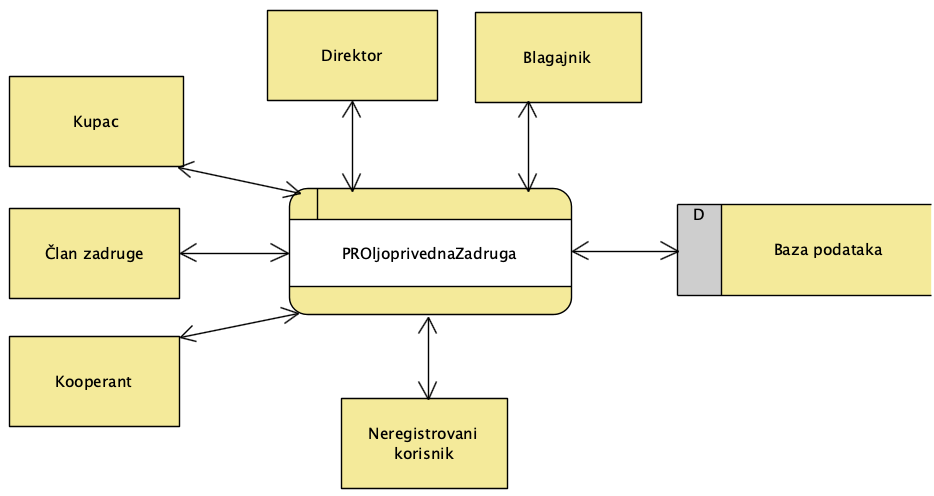
\includegraphics[scale=0.72]{images/dtp_nivo_0.png}
    \caption{DTP dijagram sistema nivoa 0}
    \label{dtp_nivo_0}
\end{figure}

\begin{figure}[h!]
    \centering
    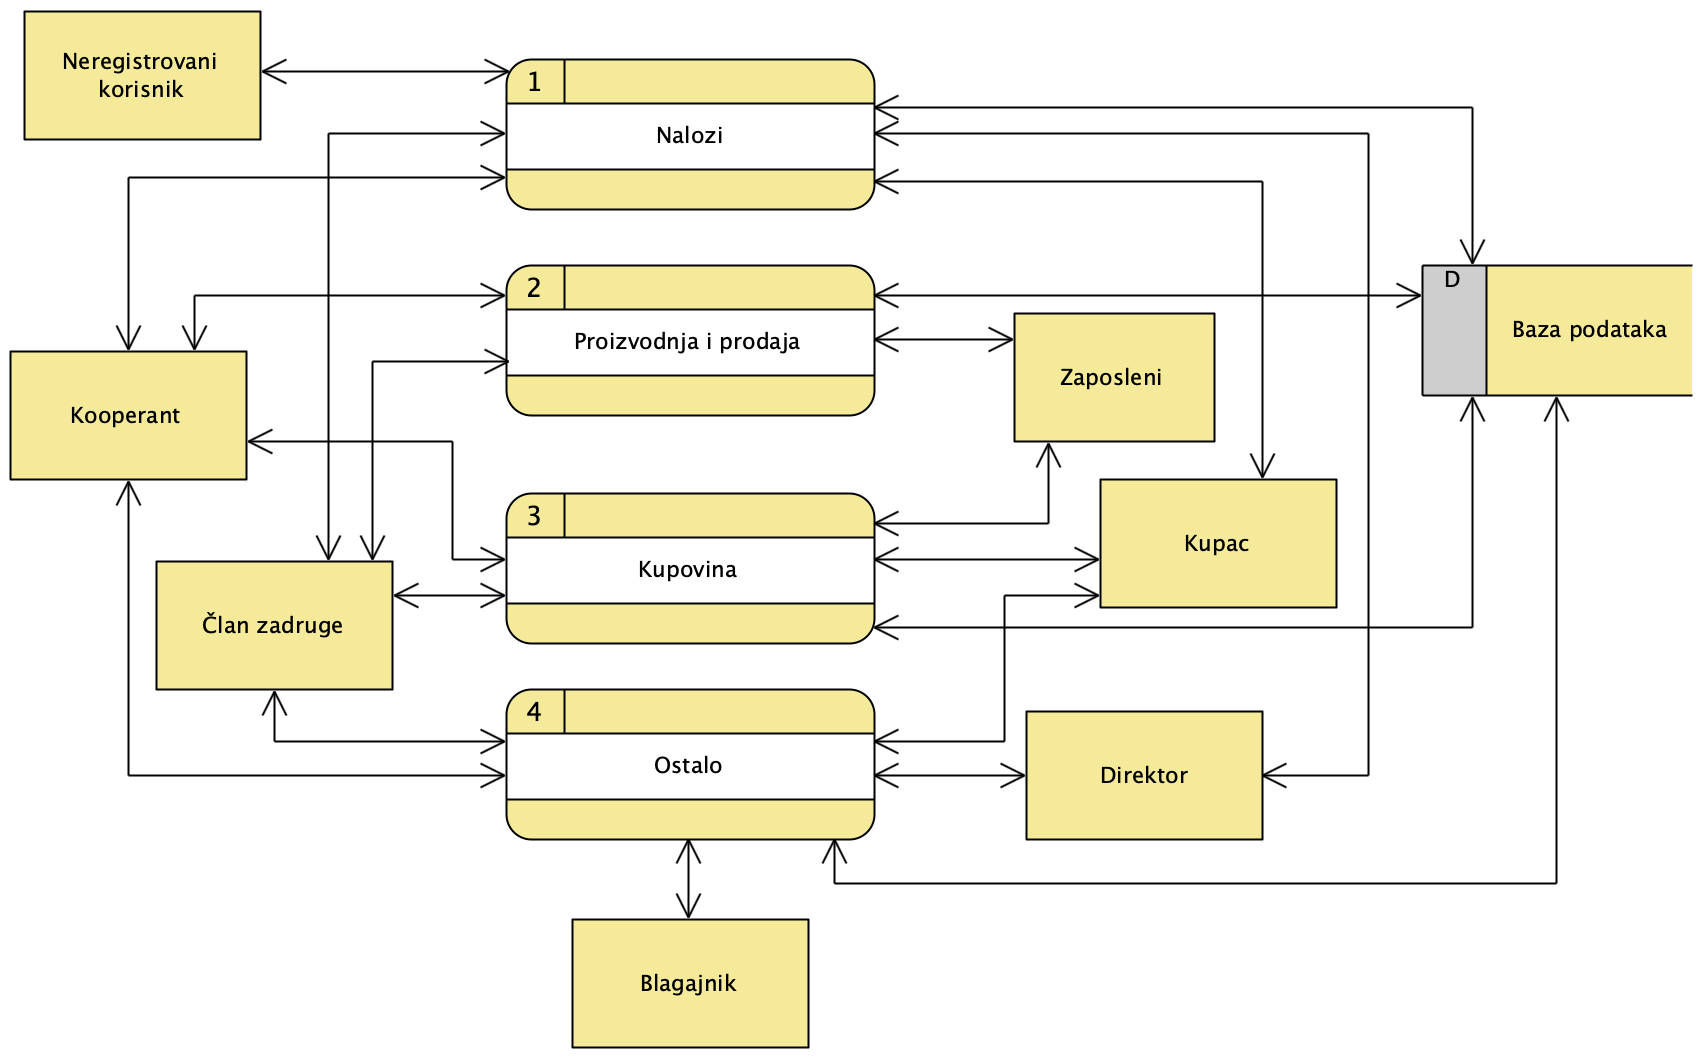
\includegraphics[scale=0.5]{images/dtp_nivo_1.png}
    \caption{DTP dijagram sistema nivoa 1}
    \label{dtp_nivo_1}
\end{figure}

\newpage

\section{Slučajevi upotrebe}

\subsection{Nalozi}
Na slici %\ref{dtp_nalozi} je prikazan dijagram toka podataka, dok je na slici 
\ref{slika1} je prikazan dijagram slucajeva upotrebe vezanih za vrste naloga u sistemu.

%\begin{figure}[h!]
%    \centering
%    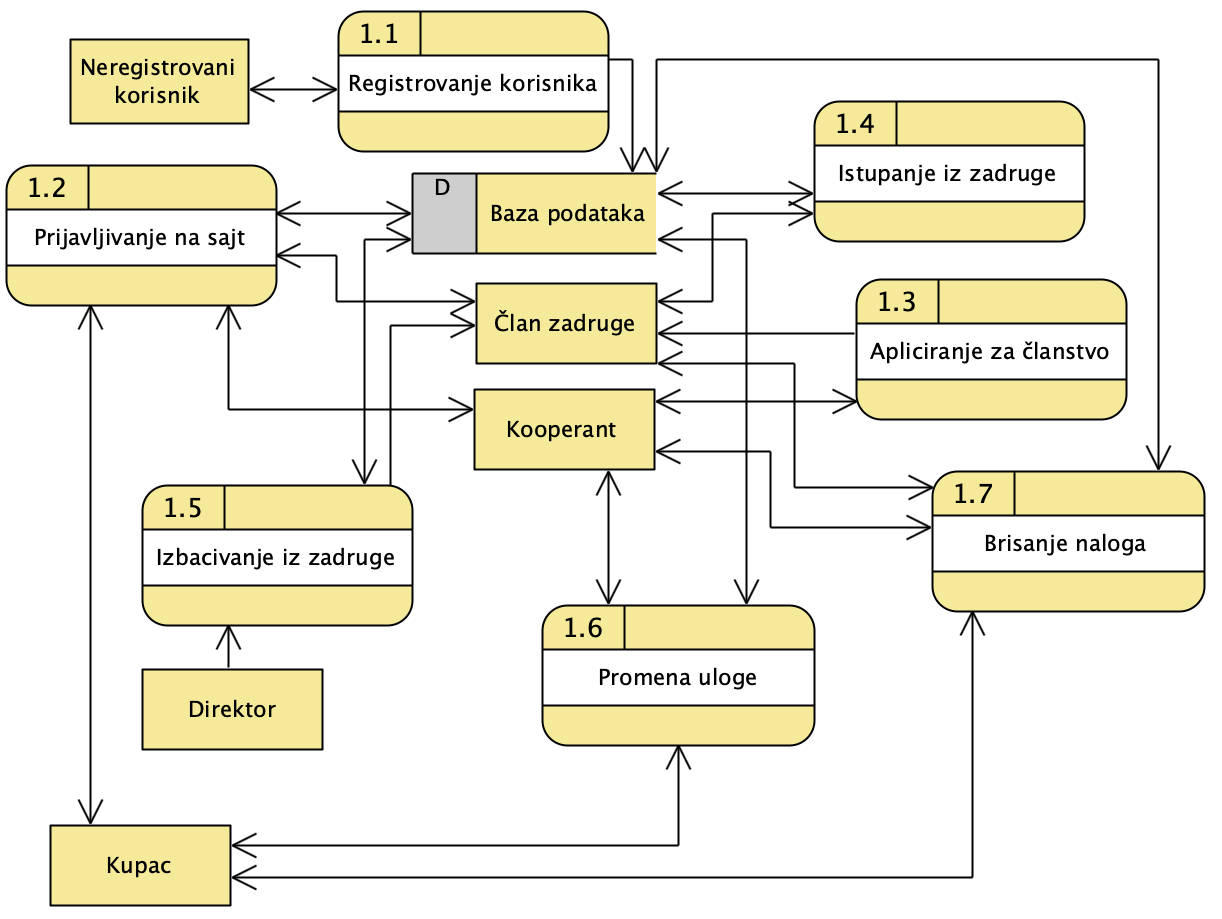
\includegraphics[scale=0.6]{images/dtp_nalozi.png}
%    \caption{Dijagram toka podataka za naloge}
%    \label{dtp_nalozi}
%\end{figure}

%\clearpage

\begin{figure}[h!]
    \centering
    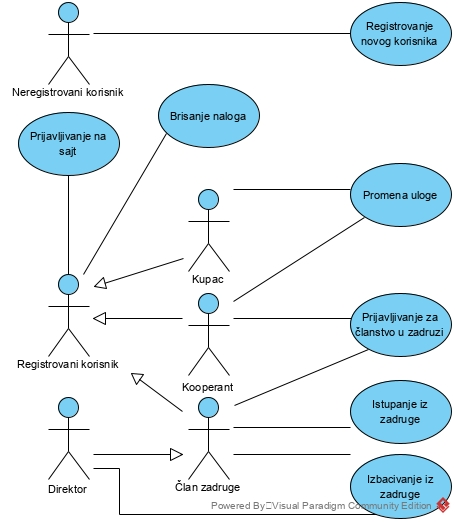
\includegraphics{images/clanstvoSU.jpg}
    \caption{Dijagram slučajeva upotrebe vezanih za vrste naloga u sistemu}
    \label{slika1}
\end{figure}

\subsubsection{Registrovanje korisnika}
Na slici \ref{dakt_registr_korisnika} je prikazan dijagram aktivnosti za proces registracije novog korisnika.
\begin{figure}[h!]
    \centering
    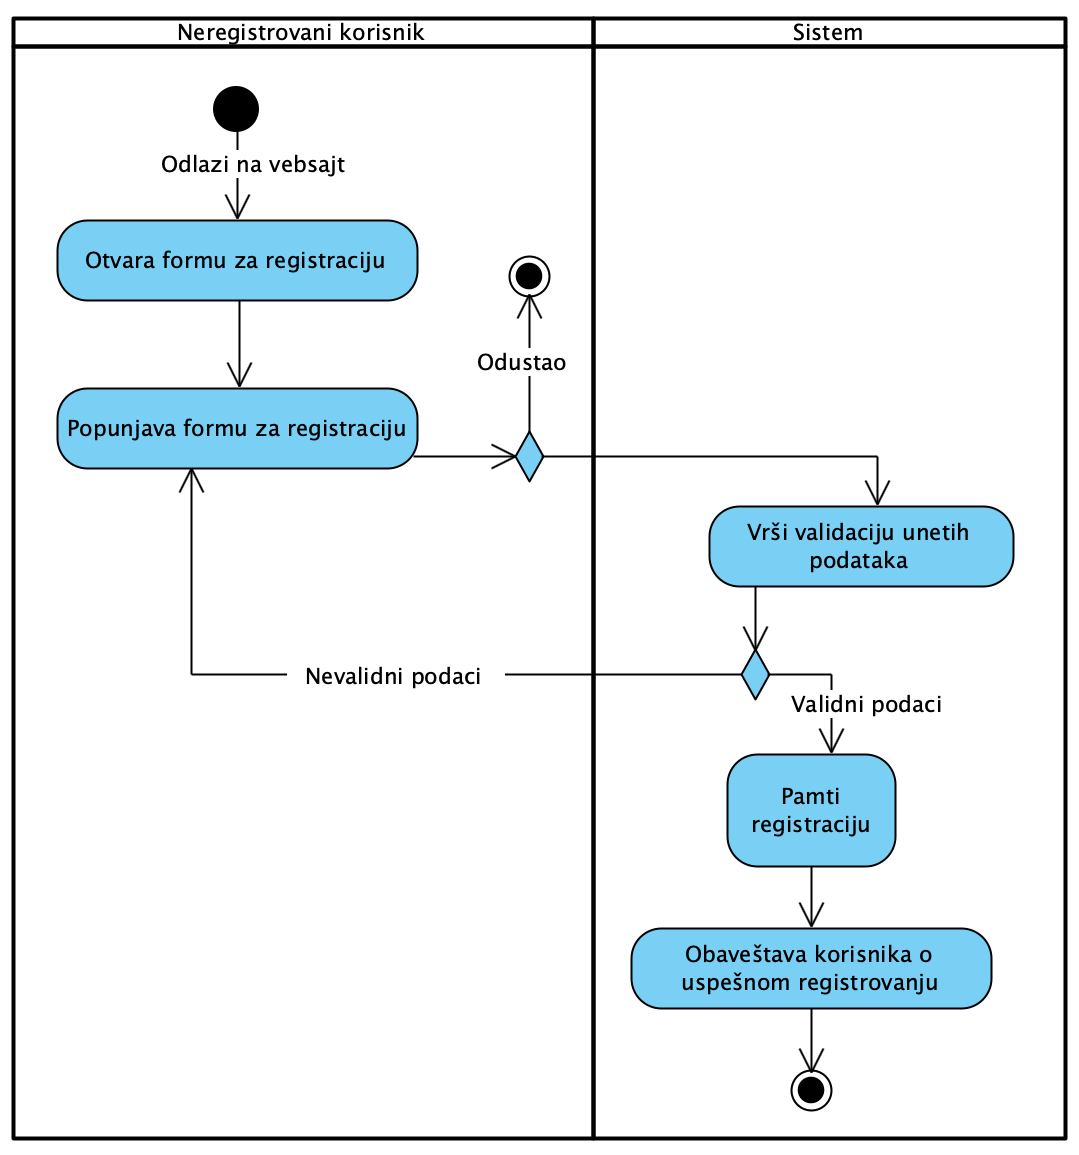
\includegraphics[scale=0.64]{images/dakt_registr_korisnika.png}
    \caption{Dijagram aktivnosti za registraciju novog korisnika}
    \label{dakt_registr_korisnika}
\end{figure}


\begin{usecase}
        \addtitle{SLUČAJ UPOTREBE}{}
        \addfield{Naziv:}{Registracija novog korisnika}
        \addfield{Kratak opis:}{Neregistrovan korisnik želi da napravi svoj nalog}
        \addfield{Učesnici:}{
            Neregistrovani korisnik 
        }
        \addfield{Preduslovi:}{
            Email adresa korisnika ne postoji u sistemu
        }
        \addfield{Postuslovi:}{
            Korisnik je uspešno registrovan u sistemu i baza podataka je ažurirana
        }

        \addscenario{Glavni tok:}{
            \item Korisnik odlazi na vebsajt i otvara formu za registraciju
            \item Korisnik popunjava formu za registraciju
            \item Korisnik bira ulogu kooperanta
            \item Korisnik popunjava dodatna polja koja se prikazuju samo budućem kooperantu 
            \item Korisnik potvrđuje svoju registraciju
            \item Sistem vrši validaciju registracije
            \item Sistem pamti unetu registraciju
            \item Sistem obaveštava korisnika o uspešnoj registraciji
        }
        \addscenario{Alternativni tokovi:}{
            \item[3.a] Ukoliko je korisnik izabrao ulogu kupca, slučaj upotrebe se nastavlja od koraka 5.
            \item[5.a] Korisnik odustaje od registracije. Slučaj upotrebe se završava.
            \item[6.a] Ukoliko je korisnik odabrao korisničko ime koje već postoji u sistemu, prikazuje se odgovarajuća poruka. Slučaj upotrebe se nastavlja od koraka 2.
            \item[6.b] Ukoliko je korisnik odabrao lozinku koja ne odgovara specifikacijama sistema (prekratka, nema nijedan broj, nema nijedno veliko slovo), prikazuje se odgovarajuća poruka. Slučaj upotrebe se nastavlja od koraka 2.
            \item[6.c] Ukoliko korisnik nije popunio sva polja forme, prikazuje se odgovarajuća poruka. Slučaj upotrebe se nastavlja od koraka 2.
            \item[6.d] Ukoliko korisnik nije izabrao ulogu koju želi da ima u sistemu, prikazuje se odgovarajuća poruka. Slučaj upotrebe se nastavlja od koraka 3.
            \item[6.e] Ukoliko korisnik nije popunio odgovarajuća polja vezana za kooperanta, prikazuje se odgovarajuća poruka. Slučaj upotrebe se nastavlja od koraka 4.
            \item[6.f] Ukoliko korisnik nije popunio odgovarajuća polja vezana za karticu, prikazuje se odgovarajuća poruka. Slučaj upotrebe se nastavlja od koraka 4.
        }
        
        \addfield{Dodatne informacije:}{Forma za prijavu sadrži sledeća polja: ime, prezime, jmbg, korisničko ime, lozinku, email adresu, broj telefona, izbor uloge u okviru sistema (kupac/kooperant) i podatke sa kartice (kreditna/debitna). Dodatna polja koja popunjava korisnik koji je izabrao ulogu kooperanta su: predmet proizvodnje, mesto proizvodnje, količina proizvoda, cena porizvoda.
        }
\end{usecase}

\subsubsection{Prijavljivanje na sajt}
\begin{usecase}
        \addtitle{SLUČAJ UPOTREBE}{}
        \addfield{Naziv:}{Prijavljivanje korisnika}
        \addfield{Kratak opis:}{Prijavljivanje već postojećeg korisnika}
        \addfield{Učesnici:}{
            Registrovani korisnik (član zadruge/kooperant/kupac) 
        }
        \addfield{Preduslovi:}{
            Korisnik je prethodno registrovan
        }
        \addfield{Postuslovi:}{
            Korisnik je uspešno pristupio svom nalogu
        }

        \addscenario{Glavni tok:}{
            \item Korisnik odlazi na vebsajt i otvara formu za prijavu
            \item Korisnik unosi korisničko ime i lozinku
            \item Korisnik potvrđuje svoj unos
            \item Sistem vrši validaciju prijave
            \item Korisnik je prijavljen na svoj nalog
        }
        \addscenario{Alternativni tokovi:}{
            \item[4.a] Ukoliko je korisnik uneo nepostojeće korisničko ime, prikazuje se odgovarajuća poruka. Slučaj upotrebe se nastavlja od koraka 2.
            \item[4.b] Ukoliko je korisnik uneo neispravnu lozinku, prikazuje se odgovarajuća poruka. Slučaj upotrebe se nastavlja od koraka 2.
        }
\end{usecase}

\subsubsection{Apliciranje za članstvo}
Na slici \ref{dakt_apliciranje_clanstvo} je prikazan dijagram aktivnosti za proces apliciranja za članstvo u zadruzi.
\begin{figure}[h!]
    \centering
    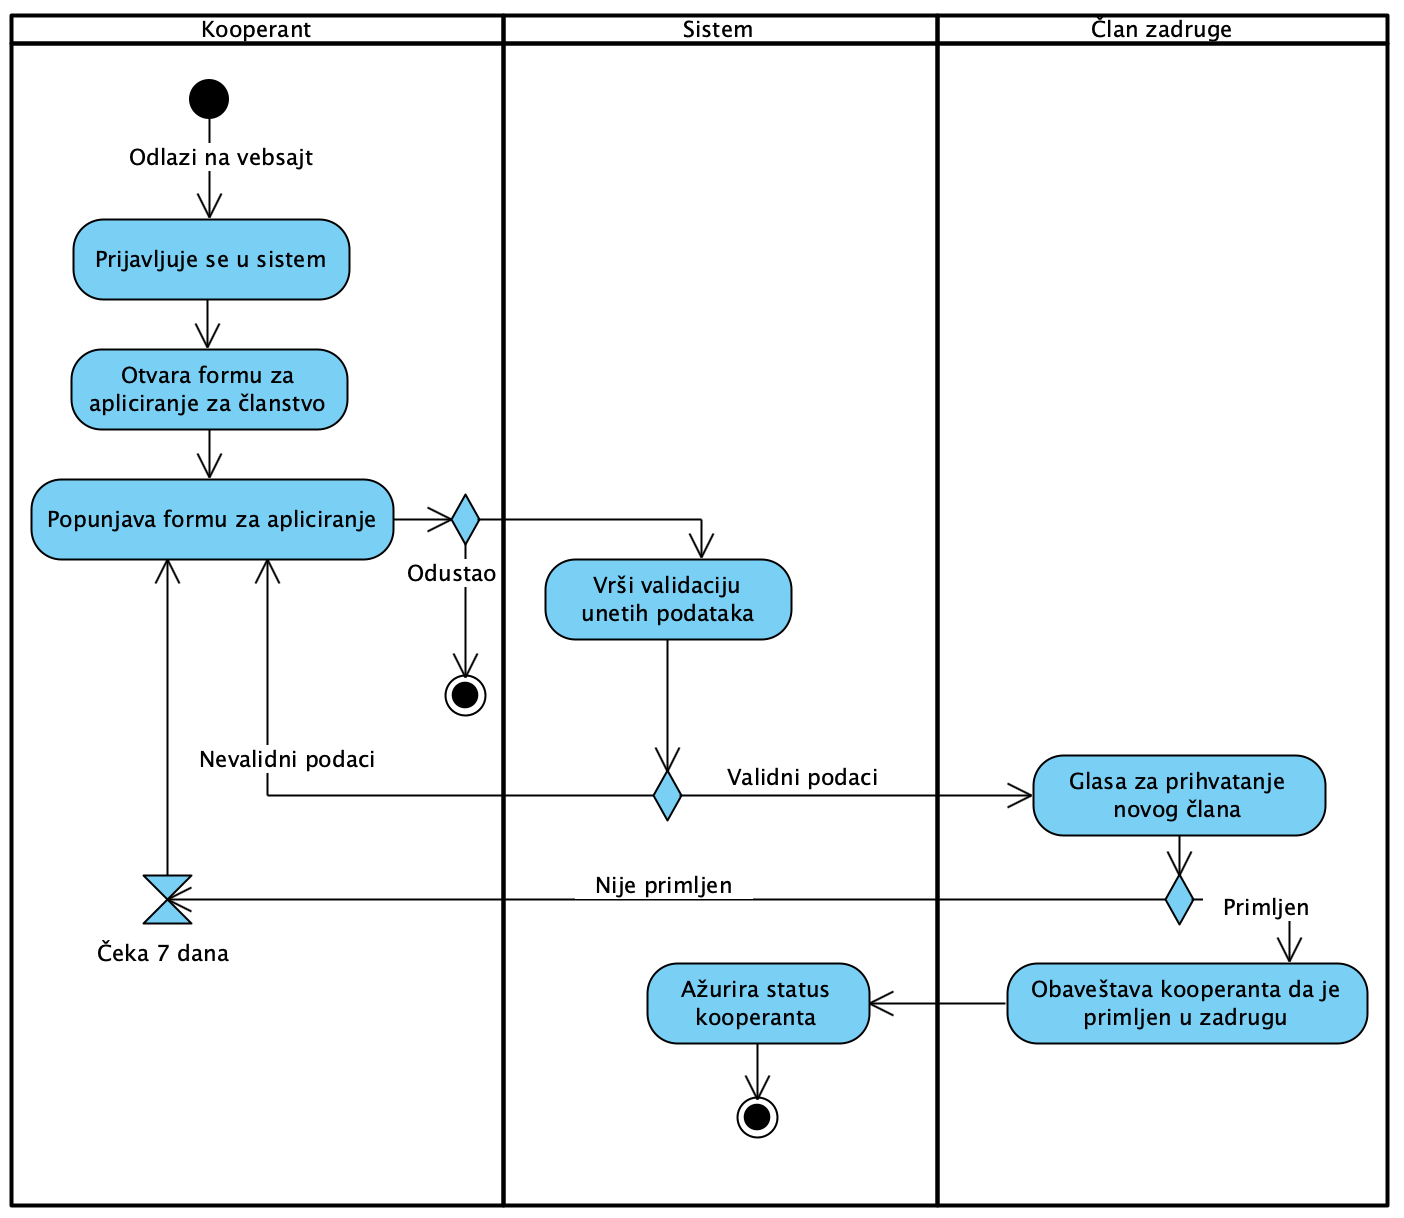
\includegraphics[scale=0.55]{images/dakt_apliciranje_clanstvo.png}
    \caption{Dijagram aktivnosti za apliciranje za članstvo u zadruzi}
    \label{dakt_apliciranje_clanstvo}
\end{figure}
\clearpage
\begin{usecase}
        \addtitle{SLUČAJ UPOTREBE}{}
        \addfield{Naziv:}{Apliciranje za članstvo u zadruzi}
        \addfield{Kratak opis:}{Kooperant, odnosno korisnik koji je registrovan u sistemu kao proizvođač šalje zahtev za učlanjivanje u zadrugu}
        \addfield{Učesnici:}{
             Kooperant, članovi zadruge
        }
        \addfield{Preduslovi:}{
            Korisnik je registrovan u sistemu kao kooperant 
        }
        \addfield{Postuslovi:}{
            Kooperant je dobio odgovor na svoj zahtev i ukoliko je potvrdan, postao je ravnopravni član zadruge
        }

        \addscenario{Glavni tok:}{
            \item Kooperant odlazi na vebsajt i prijavljuje se
            \item Kooperant popunjava podatke neophodne za apliciranje za članstvo u zadruzi
            \item Kooperant šalje zahtev na obradu
            \item Sistem vrši validaciju prijave
            \item Sistem prihvata zahtev za članstvo i prosleđuje ga članovima zadruge 
            \item Članovi zadruge imaju rok od 72h da izvrše glasanje za prihvatanje novog člana
            \item Sistem obaveštava kooperanta da je primljen u zadrugu
            \item Uloga trenutnog korisnika je promenjena u sistemu i on je sada ravnopravni član zadruge 
        }
        \addscenario{Alternativni tokovi:}{
            \item[3.a] Kooperant odustaje od apliciranja za članstvo. Slučaj upotrebe se završava.
            \item[4.a] Ukoliko kooperant nije uneo sve potrebne podatke i/ili podaci nisu u traženom formatu, prikazuje se odgovarajuća poruka. Slučaj upotrebe se nastavlja od koraka 2.
            \item[7.a] Ukoliko kooperant nije primljen u zadrugu, ostaje kooperant i može se ponovo prijaviti za nedelju dana. Slučaj upotrebe se završava.
        }
        \addfield{Dodatne informacije:}{
            Informacije koje kooperant unosi u zahtevu za članstvo su: razlog za pristupanje zadruzi, vremenski period u ulozi kooperanta zadruge, proizvodi prodavani zadruzi, dodatni proizvodi koje bi mogao da prodaje, način doprinosa zadruzi.
        }
\end{usecase}


\subsubsection{Istupanje iz zadruge}
\begin{usecase}
        \addtitle{SLUČAJ UPOTREBE}{}
        \addfield{Naziv:}{Istupanje iz zadruge}
        \addfield{Kratak opis:}{Član zadruge želi da istupi iz iste uz mogućnost odabira svoje uloge u sistemu kooperant/kupac/potpuno brisanje naloga}
        \addfield{Učesnici:}{
             Član zadruge
        }
        \addfield{Preduslovi:}{
           Korisnik je član zadruge
        }
        \addfield{Postuslovi:}{
           Korisnik više nije član zadruge
        }

        \addscenario{Glavni tok:}{
            \item Član zadruge odlazi na vebsajt i prijavljuje se
            \item Član zadruge odabira opciju napuštanja zadruge 
            \item Član zadruge unosi razlog za napuštanje zadruge 
            \item Član zadruge odabira brisanje naloga kao novu ulogu unutar sistema
            \item Član zadruge šalje popunjeni zahtev 
            \item Sistem obrađuje zahtev 
            \item Menja se uloga korisnika u bazi podataka
            \item Korisnik dobija poruku o uspešnom napuštanju zadruge
        }
        \addscenario{Alternativni tokovi:}{
            \item[4.a] Član zadruge je izabrao da postane kooperant, sistem obrađuje zahtev i obaveštava korisnika da od sada ima ulogu kooperanta. Slučaj upotrebe se završava.
            \item[4.b] Član zadruge je izabrao da postane kupac, sistem obrađuje zahtev i obaveštava korisnika da od sada ima ulogu kupca. Slučaj upotrebe se završava.
            \item[5.a] Član zadruge je ipak rešio da ostane član (napuštanjem forme ili poništavanjem unetih podataka), slučaj upotrebe se završava.
    
        }
\end{usecase}

\subsubsection{Izbacivanje iz zadruge}

Na slici \ref{dsekv_izbacivanje_iz_zadruge} je prikazan dijagram sekvence izbacivanja člana iz zadruge.
\begin{figure}[h!]
    \centering
    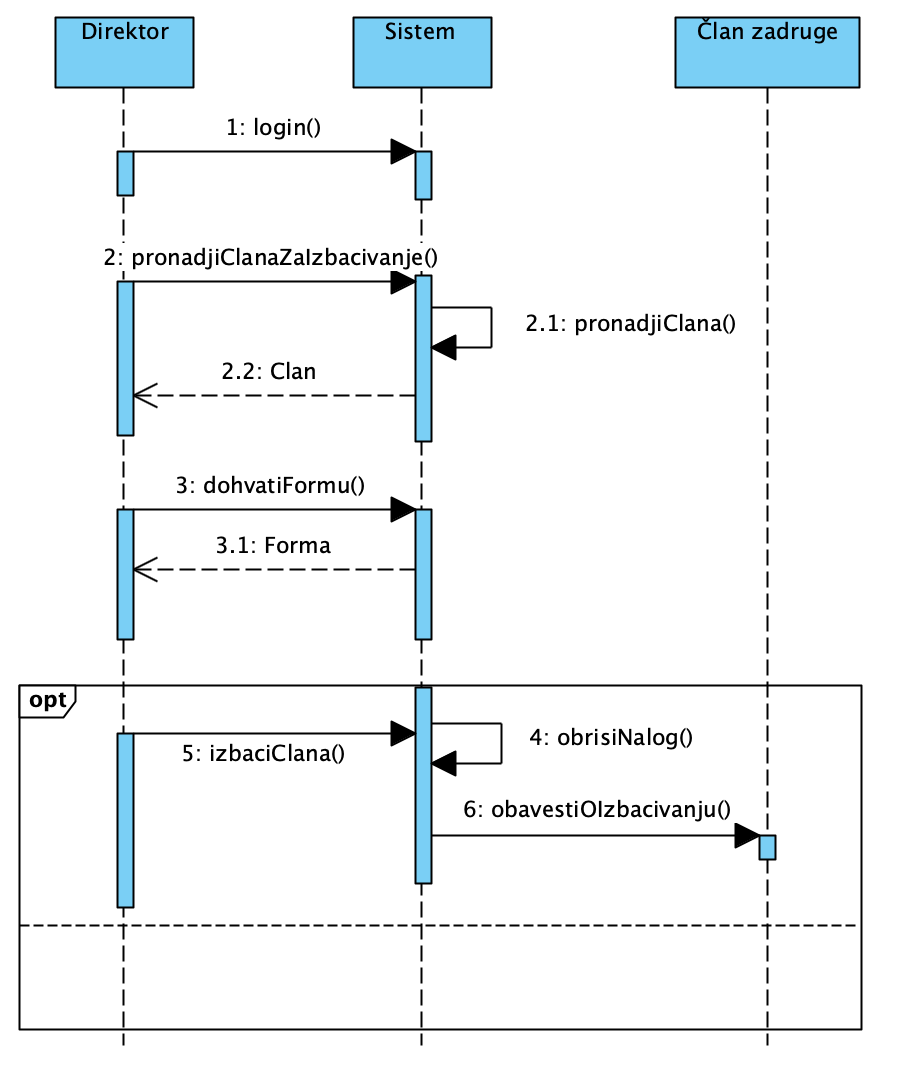
\includegraphics[scale=0.7]{images/dsekv_izbacivanje_iz_zadruge.png}
    \caption{Dijagram sekvence izbacivanja člana iz zadruge}
    \label{dsekv_izbacivanje_iz_zadruge}
\end{figure}
\clearpage

\begin{usecase}
        \addtitle{SLUČAJ UPOTREBE}{}
        \addfield{Naziv:}{Izbacivanje člana iz zadruge}
        \addfield{Kratak opis:}{Član zadruge je prekršio neko od osnovnih pravila i direktor zadruge je rešio da ga izbaci iz iste}
        \addfield{Učesnici:}{
            Član zadruge, direktor
        }
        \addfield{Preduslovi:}{
           Korisnik je član zadruge i prekršio je neko od osnovnih pravila
        }
        \addfield{Postuslovi:}{
           Korisnik više nije član zadruge i ne može se prijaviti za u istu u narednih godinu dana
        }

        \addscenario{Glavni tok:}{
            \item Direktor zadruge odlazi na vebsajt i prijavljuje se
            \item Direktor pronalazi odgovarajućeg korisnika u sistemu i prelazi na formu za izbacivanje člana iz zadruge
            \item Direktor unosi razlog ga izbacivanje člana iz zadruge, odnosno bira koje je pravilo prekršio član zadruge
            \item Direktor potvrđuje unesene podatke
            \item Sistem obrađuje zahtev
            \item Sistem briše člana zadruge
            \item Sistem šalje poruku korisniku na email adresu koja sadrži razlog izbacivanja i obaveštenje da je njegov nalog izbrisan
        }
        \addscenario{Alternativni tokovi:}{
            \item[4.a] Direktor je rešio da ne izbaci člana iz zadruge (napuštanjem forme ili poništavanjem unetih podataka), slučaj upotrebe se završava.
        }
\end{usecase}


\subsubsection{Promena uloge}
\begin{usecase}
        \addtitle{SLUČAJ UPOTREBE}{}
        \addfield{Naziv:}{Promena uloge korisnika sistema}
        \addfield{Kratak opis:}{Korisnik koji ima ulogu kupca/kooperanta želi da postane kooperant/kupac}
        \addfield{Učesnici:}{
            Kooperant, kupac
        }
        \addfield{Preduslovi:}{
           Korisnik je registrovan u sistemu i nije član zadruge
        }
        \addfield{Postuslovi:}{
           Uloga korisnika u sistemu je uspešno promenjena i baza podataka je ažurirana
        }

        \addscenario{Glavni tok:}{
            \item Korisnik odlazi na vebsajt i prijavljuje se
            \item Korisnik prelazi na formu za promenu uloge
            \item Korisnik unosi razlog za promenu uloge 
            \item Korisnik je trenutno kupac i izabrao je da želi postati kooperant
            \item Korisnik popunjava preostala dodatna polja
            \item Korisnik potvrđuje unesene podatke
            \item Sistem obrađuje zahtev
            \item Uloga korisnika je uspešno promenjena u sistemu
        }
        \addscenario{Alternativni tokovi:}{
            \item[4.a] Ukoliko je korisnik trenutno kooperant i izabrao je da postane kupac. Slučaj upotrebe se nastavlja od koraka 5.
            \item[7.a] Ukoliko korisnik nije popunio dodatna polja, prikazuje se obaveštenje sa informacijom koja su polja obavezna. Slučaj upotrebe se nastavlja od koraka 5.
        }
        \addfield{Dodatne informacije:}{
           Dodatna polja koja popunjava kupac koji želi postati kooperant: predmet proizvodnje, mesto proizvodnje, količina proizvodnje, cena proizvoda.
        }
\end{usecase}

\subsubsection{Brisanje naloga}
\begin{usecase}
        \addtitle{SLUČAJ UPOTREBE}{}
        \addfield{Naziv:}{Brisanje naloga iz sistema}
        \addfield{Kratak opis:}{Korisnik želi da obriše svoj nalog}
        \addfield{Učesnici:}{
            Registrovani korisnik (član zadruge/kooperant/kupac)
        }
        \addfield{Preduslovi:}{
           Korisnik je registrovan u sistemu
        }
        \addfield{Postuslovi:}{
           Nalog korisnika je uspešno obrisan i njegova email adresa je izbrisana iz baze podataka
        }

        \addscenario{Glavni tok:}{
            \item Korisnik odlazi na vebsajt i prijavljuje se
            \item Korisnik prelazi na formu za brisanje naloga
            \item Korisnik unosi razlog brisanja naloga
            \item Korisnik potvrđuje unesene podatke 
            \item Korisnik šalje zahtev sistemu
            \item Sistem obrađuje zahtev
            \item Nalog korisnika je uspešno obrisan iz sistema
        }
        \addscenario{Alternativni tokovi:}{
            \item[2.a] Trenutni korisnik je član zadruge. Dobija poruku da se prvo mora isčlaniti iz zadruge i biva preusmeren na slučaj upotrebe \hyperref[subsubsec:istupanjeIzZadruge]{'Istupanje iz zadruge'}. Slučaj upotrebe se završava.
            \item[4.a] Ukoliko je korisnik ipak rešio da ne obriše nalog (napuštanjem forme ili poništavanjem unetih podataka), slučaj upotrebe se završava.
        }
\end{usecase}


\subsection{Proizvodnja i prodaja}

Na slici %\ref{dtp_proizvodnja_prodaja} je prikazan dijagram toka podataka za slučaj upotrebe proizvodnja i prodaja, dok je na slici 
\ref{dslucup_proizvodnja_prodaja} je prikazan dijagram slučajeva upotrebe proizvodnja i prodaja.

%\begin{figure}[h!]
%    \centering
%    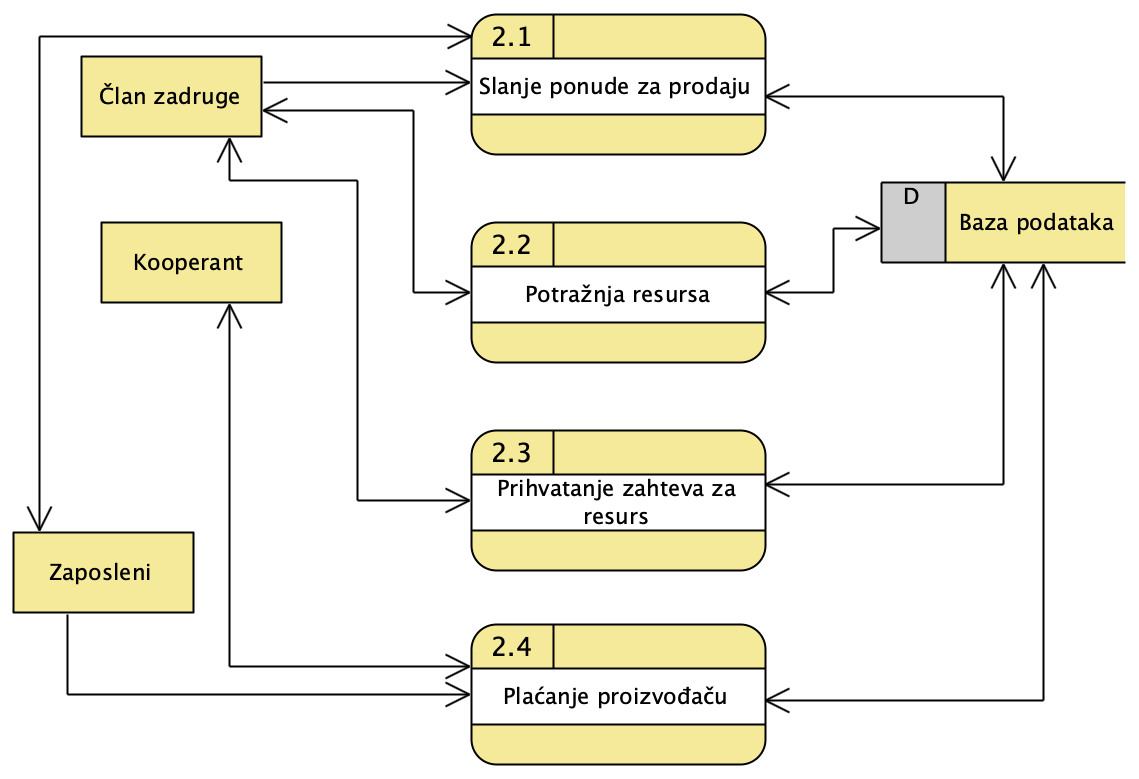
\includegraphics[scale=0.64]{images/dtp_proizvodnja_prodaja.png}
%    \caption{Dijagram toka podataka za slučaj upotrebe proizvodnja i prodaja}
%    \label{dtp_proizvodnja_prodaja}
%\end{figure}

\begin{figure}[h!]
    \centering
    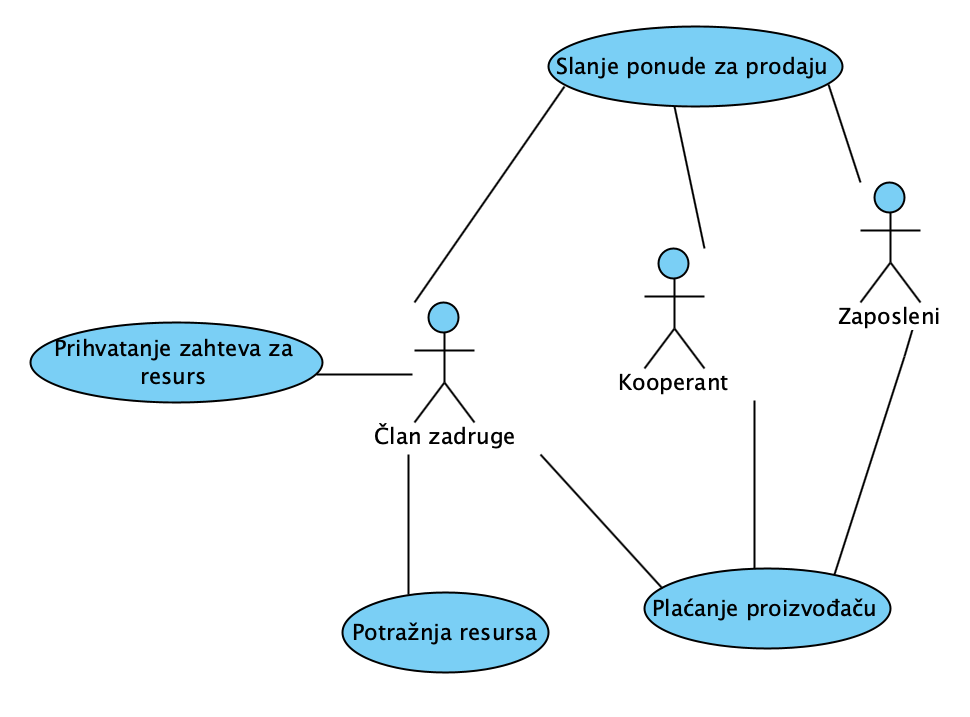
\includegraphics[scale=0.64]{images/dslucup_proizvodnja_prodaja.png}
    \caption{Dijagram slučaja upotrebe vezanog za proizvodnju i prodaju}
    \label{dslucup_proizvodnja_prodaja}
\end{figure}

\clearpage

\subsubsection{Slanje ponude za prodaju}

Na slici \ref{dakt_slanje_ponude_za_prodaju} je prikazan dijagram aktivnosti za proces slanja ponude za prodaju proizvoda.
\begin{figure}[h!]
    \centering
    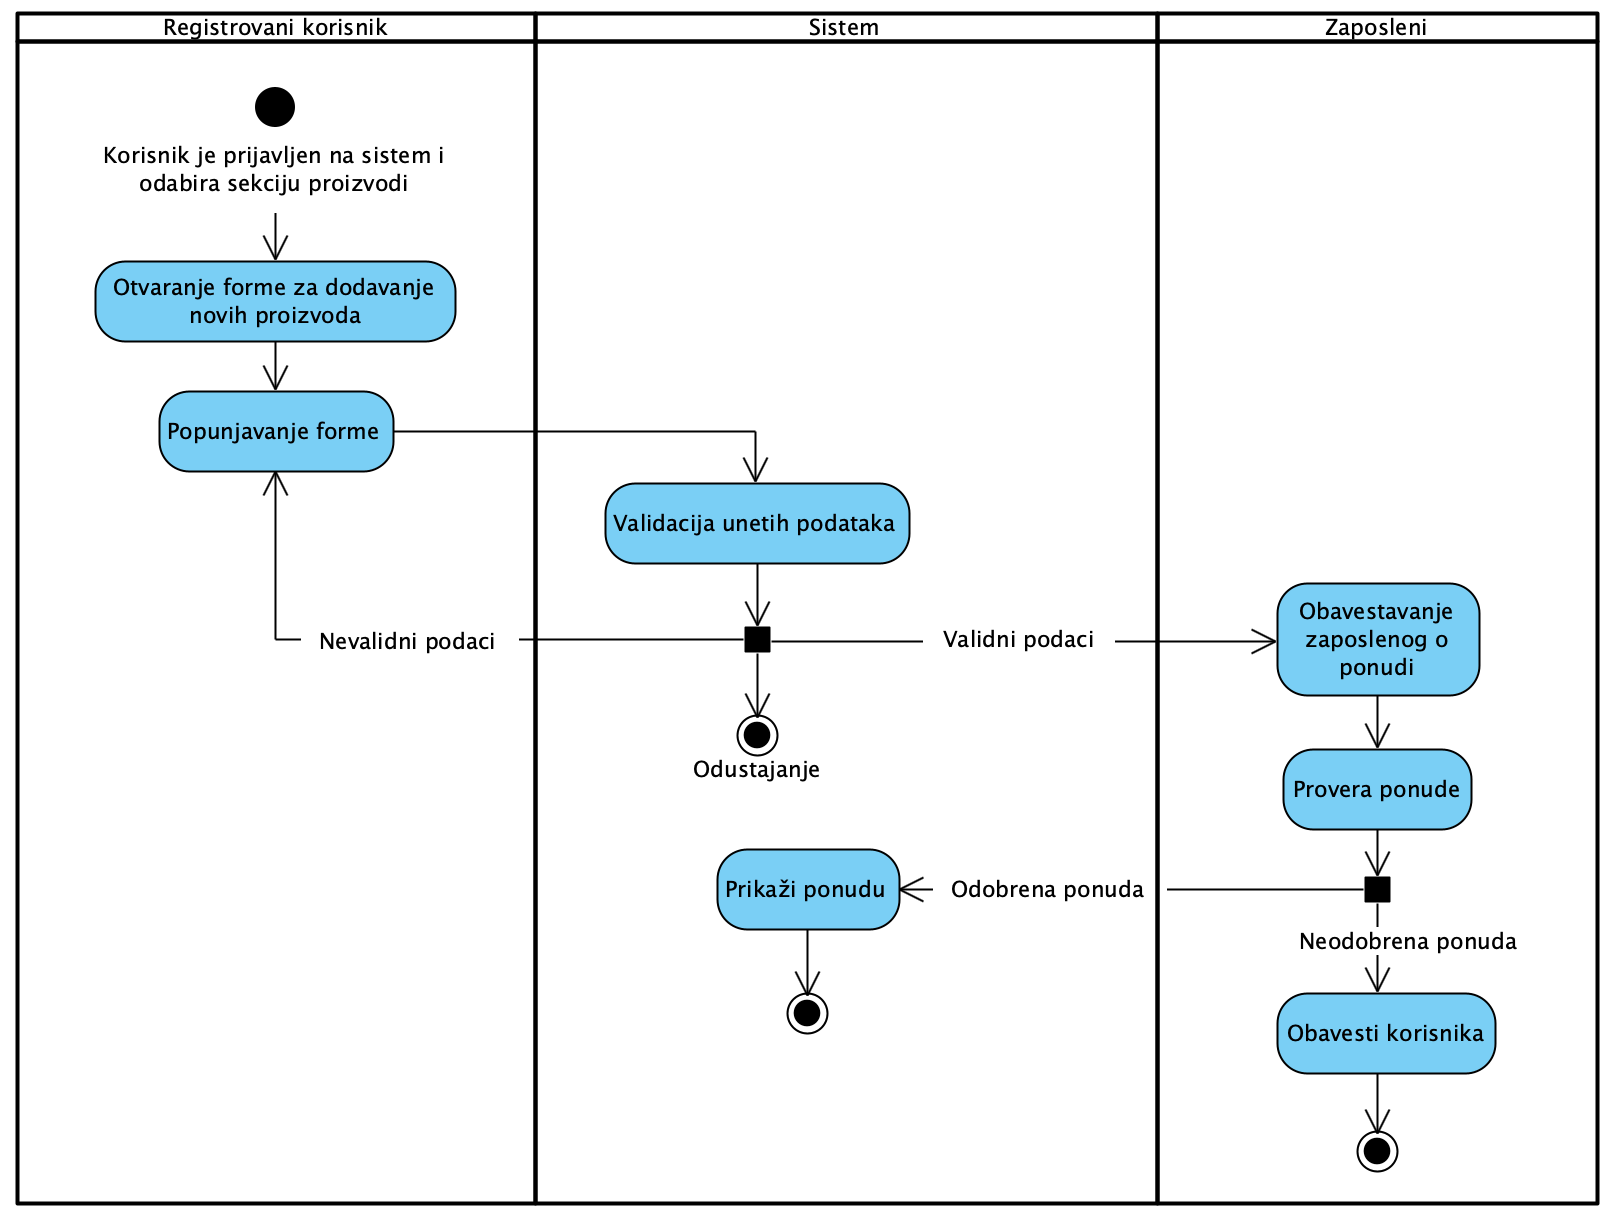
\includegraphics[scale=0.5]{images/dakt_slanje_ponude_za_prodaju.png}
    \caption{Dijagram aktivnosti za slanje ponude za prodaju proizvoda}
    \label{dakt_slanje_ponude_za_prodaju}
\end{figure}


\begin{usecase}
        \addtitle{SLUČAJ UPOTREBE}{}
        \addfield{Naziv:}{Slanje ponude za prodaju zahteva}
        \addfield{Kratak opis:}{Korisnik šalje podatke o trenutnom stanju proizvoda koji su dostupni za prodaju}
        \addfield{Učesnici:}{
        Član zadruge, kooperant, zaposleni zadruge
        }
        \addfield{Preduslovi:}{
        Korisnik je registrovan i ima ulogu člana zadruge ili kooperanta
        }
        \addfield{Postuslovi:}{
        Proizvodi su prikazani potencijalnim kupcima kao deo ponude zadruge
        }

        \addscenario{Glavni tok:}{
            \item Korisnik se nalazi na sekciji proizvodi
            \item Korisnik izabira opciju za dodavanje novih proizvoda ponudi
            \item Korisnik popunjava formu sa opisom, cenom i kolicinom dostupnih proizvoda
            \item Korisnik potvrđuje podatke
            \item Sistem validira upisane podatke
            \item Sistem obaveštava zaposlenog zadruge o ponudi
            \item Zaposleni zadruge proverava ponudu i odobrava je
            \item Sistem prikazuje ponudu kao deo ponude zadruge
        }
        \addscenario{Alternativni tokovi:}{
            \item[5.a] Ukoliko podaci nisu validni slučaj upotrebe se nastavlja od koraka 3
            
            \item[7.a] Ukoliko zaposleni zadruge ne odobri ponudu, ponuda se briše, kooperant ili član zadruge se obaveštava i slučaj upotrebe se završava
            
        }
\end{usecase}


\subsubsection{Potražnja resursa}
\begin{usecase}
        \addtitle{SLUČAJ UPOTREBE}{}
        \addfield{Naziv:}{Potraživanje resursa}
        \addfield{Kratak opis:}{Član zadruge potražuje resurs od drugih članova zadruge u vidu materijala, mašina ili skladišta}
        \addfield{Učesnici:}{
        Članovi zadruge
        }
        \addfield{Preduslovi:}{
        Korisnik je registrovan i aktivni je član zadruge
           
        }
        \addfield{Postuslovi:}{
        Korisnik je objavio potražnju za resursom
        }

        \addscenario{Glavni tok:}{
            \item Korisnik prelazi na formu za potraživanje resursa
            \item Korisnik izabira mašinu kao vrstu resursa za potražnju
            \item Korisnik popunjava formu koja sadži informacije o traženoj mašini
            \item Korisnik unosi podatke o nadoknadi koju nudi za željeni resurs
            \item Sistem vrši validaciju podataka
            \item Sistem formira oglas i obaveštava članove zadruge o novom oglasu
            \item Sistem obaveštava korisnika o uspešnoj potražnji
            
        }
        \addscenario{Alternativni tokovi:}{
            \item[2.a] Ukoliko korisnik izabere skladište kao resurs za potražnju, forma za taj resurs se popunjava i slučaj upotrebe se nastavlja od koraka 4
            
            \item[2.b] Ukoliko korisnik izabere materijale kao resurs za potražnju, forma za taj resurs se popunjava i slučaj upotrebe se nastavlja od koraka 4
            
            \item[2.c] Ukoliko korisnik izabere uslugu kao resurs za potražnju, forma za taj resurs se popunjava i slučaj upotrebe se nastavlja od koraka 4
            
            \item[5.b] Ukoliko neki od traženih podataka nije unesen ili nije valida slučaj upotrebe se vraća na korak 2
            
        }
        
        \addfield{Dodatne informacije:}{
        Forma koja se tiče potražnje mašina sadrži podatke o tipu i modelu mašine kao i o vremenskoj odrednici za koju se mašina potražuje
        
        Forma koja se tiče potražnje materijala sadrži podatke o vrsti i količini materijala za obradu
        
        Forma koja se tiče potražnje usluge kao što je pomoć oko obrade sadrži o vrsti i trajanju usluge
        
        Forma koja se tiče potražnje sladišta sadrži podatke o veličini i okvirnoj lokaciji traženog skladišta
        }
\end{usecase}



\subsubsection{Prihvatanje zahteva za resurs}
\begin{usecase}
        \addtitle{SLUČAJ UPOTREBE}{}
        \addfield{Naziv:}{Prihvatanje zahteva za resurs}
        \addfield{Kratak opis:}{Član zadruge prihvata zahtev za resurs i povezuje se sa drugim članom radi daljih pregovora}
        \addfield{Učesnici:}{
        Članovi zadruge
        }
        \addfield{Preduslovi:}{
        Korisnik je registrovan i aktivni je član zadruge
        }
        \addfield{Postuslovi:}{
        Sistem je povezao članove radi daljih pregovora oko traženog resursa
        }

        \addscenario{Glavni tok:}{
            \item Korisnik pretražuje postojeće oglase
            \item Korisnik izabira oglas za koji je zainteresovan 
            \item Korisnik popunjava formu za oglas za koji je zainteresovan
            \item Sistem vrši validaciju podataka
            \item Sistem šalje podatke korisniku koji potražuje resurs
            \item Korisnik prihvata postojeću ponudu
            \item Sistem obaveštava korisnika o uspešnoj saradnji i omogućava dalju komunikaciju korisnika
            
        }
        \addscenario{Alternativni tokovi:}{
            \item[6.a] Ukoliko član zadruge ne prihvati ponudu korisnika sistem obaveštava korisnika o tome, i slušaj upotrebe se završava
            
            \item[6.b] Ukoliko član zadruge ne odgovori na ponudu u roku od 72 sata, sistem obaveštava korisnika o tome, oglas se privremeno uklanja i slušaj upotrebe se završava
            
        }
        
        \addfield{Dodatne informacije:}{
        Forma koju korisnik popunjava zavisi od vrste resursa pa sadrži tip mašine, vreme proizvodnje, trajanje usloge ili vrstu skladišta, veličinu itd.
        }
\end{usecase}

\subsubsection{Plaćanje proizvođaču}

Na slici \ref{dsekv_placanje_proizvodjacu} je prikazan dijagram sekvence plaćanja proizvođaču.
\begin{figure}[h!]
    \centering
    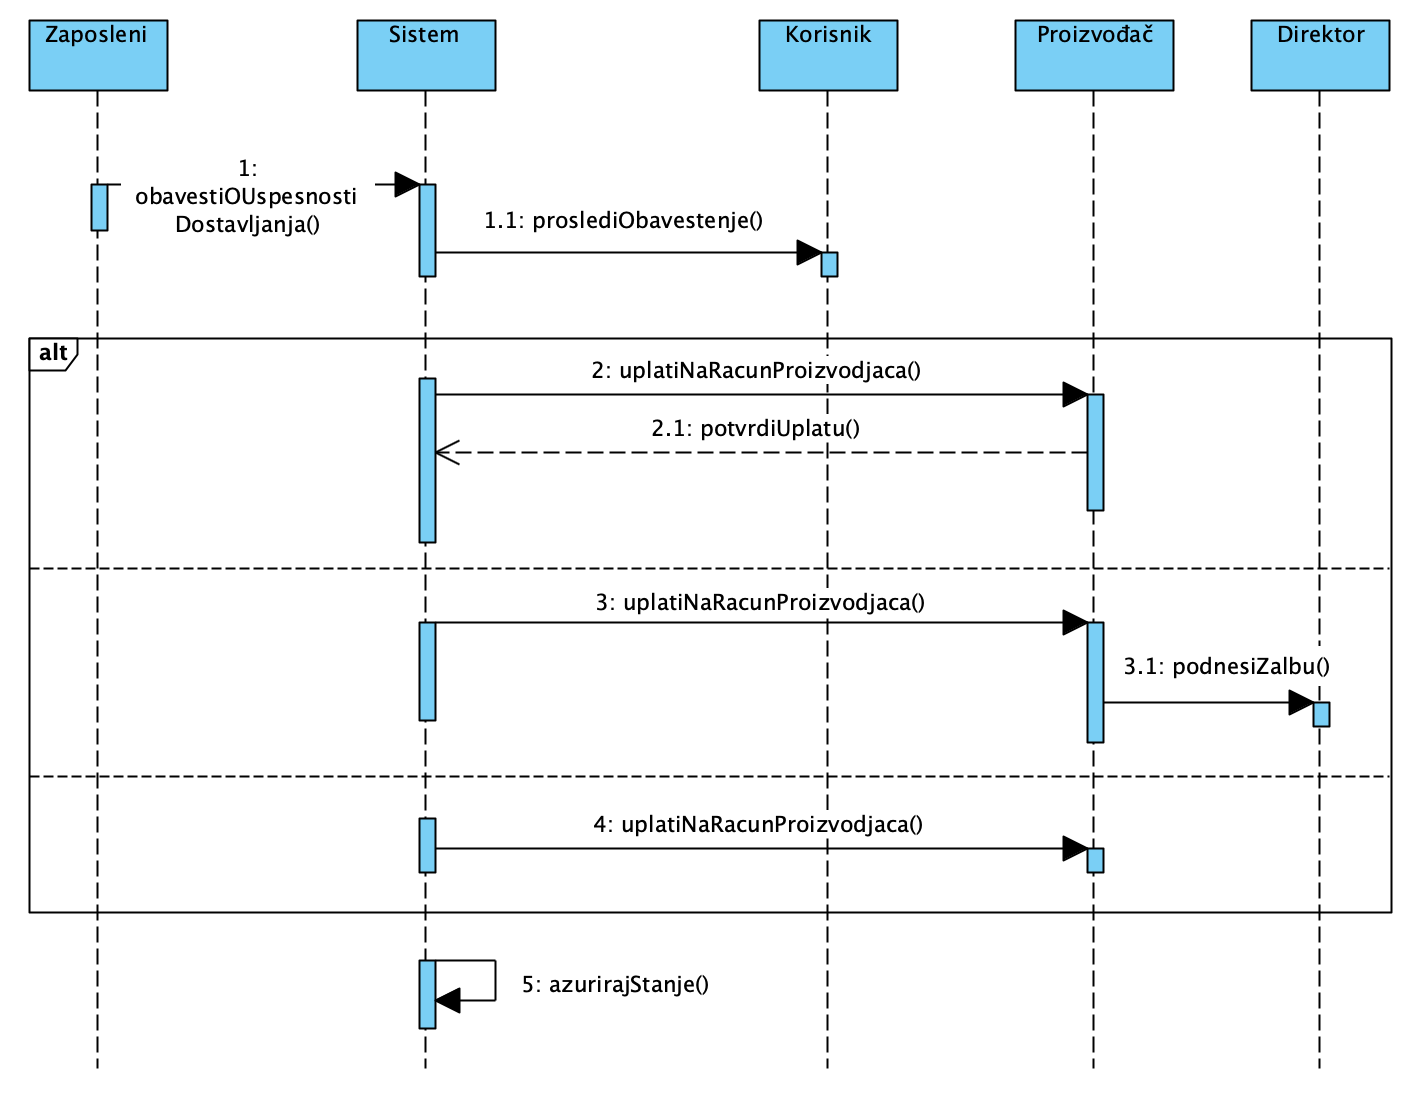
\includegraphics[scale=0.55]{images/dsekv_placanje_proizvodjacu.png}
    \caption{Dijagram sekvence plaćanja proizvođaču}
    \label{dsekv_placanje_proizvodjacu}
\end{figure}
\clearpage

\begin{usecase}
        \addtitle{SLUČAJ UPOTREBE}{}
        \addfield{Naziv:}{Plaćanje proizvođaču}
        \addfield{Kratak opis:}{Nakon što je roba isporučena i plaćena, korisniku su resursi plaćeni}
        \addfield{Učesnici:}{
            Kooperant, član zadruge, zaposleni zadruge
        }
        \addfield{Preduslovi:}{
            Proizvodi su plaćeni, dostavljeni i stanje na računu je odgovarajuće
           
        }
        \addfield{Postuslovi:}{
           Proizvođaču je isplaćen novac za prodate proizvode
        }

        \addscenario{Glavni tok:}{
            \item Zaposleni obaveštava sistem da su proizvodi uspešno dostavljeni
            \item Sistem obaveštava korisnika o uspešnoj dostavi
            \item Sistem uplaćuje sredstva na račun proizvođača uz uračunatu proviziju
            \item Sistem ažurira stanje računa
            \item Proizvođač je obavešten o uplati
            \item Proizvođač potvrđuje da je uplata uspešno izvršena
            
        }
        \addscenario{Alternativni tokovi:}{
            \item[6.a] Prozivođač ne potvrđuje da je uplata uspešno izvršena,  ulaže žalbu koja se šalje direktoru. Slučaj upotrebe se završava 
        }
\end{usecase}


\subsection{Kupovina}

Na slici %\ref{dtp_kupovina} je prikazan dijagram toka podataka za slučaj kupovina, dok je na slici 
\ref{dslucup_kupovina} je prikazan dijagram slučajeva upotrebe kupovina.
%\begin{figure}[h!]
%    \centering
%    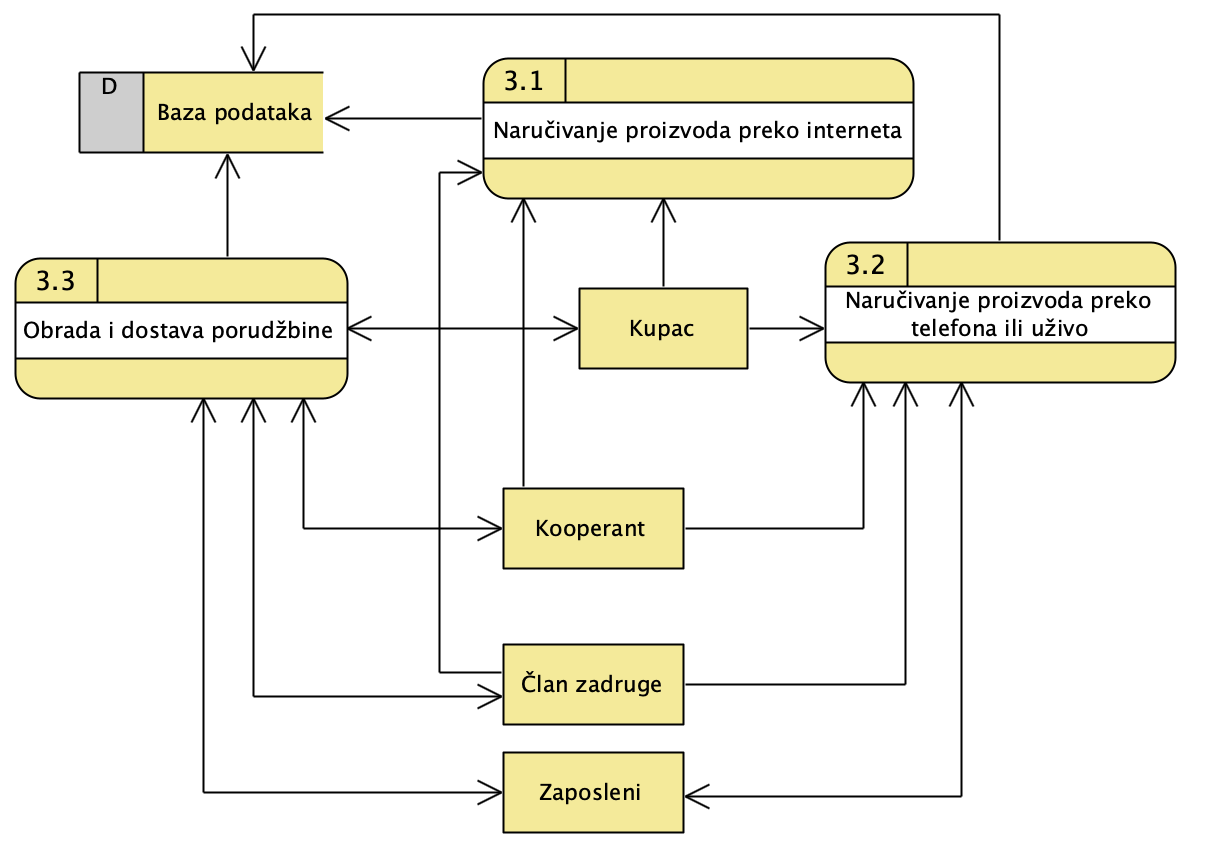
\includegraphics[scale=0.64]{images/dtp_kupovina.png}
%    \caption{Dijagram toka podataka za slučaj upotrebe kupovina}
%    \label{dtp_kupovina}
%\end{figure}

\begin{figure}[h!]
    \centering
    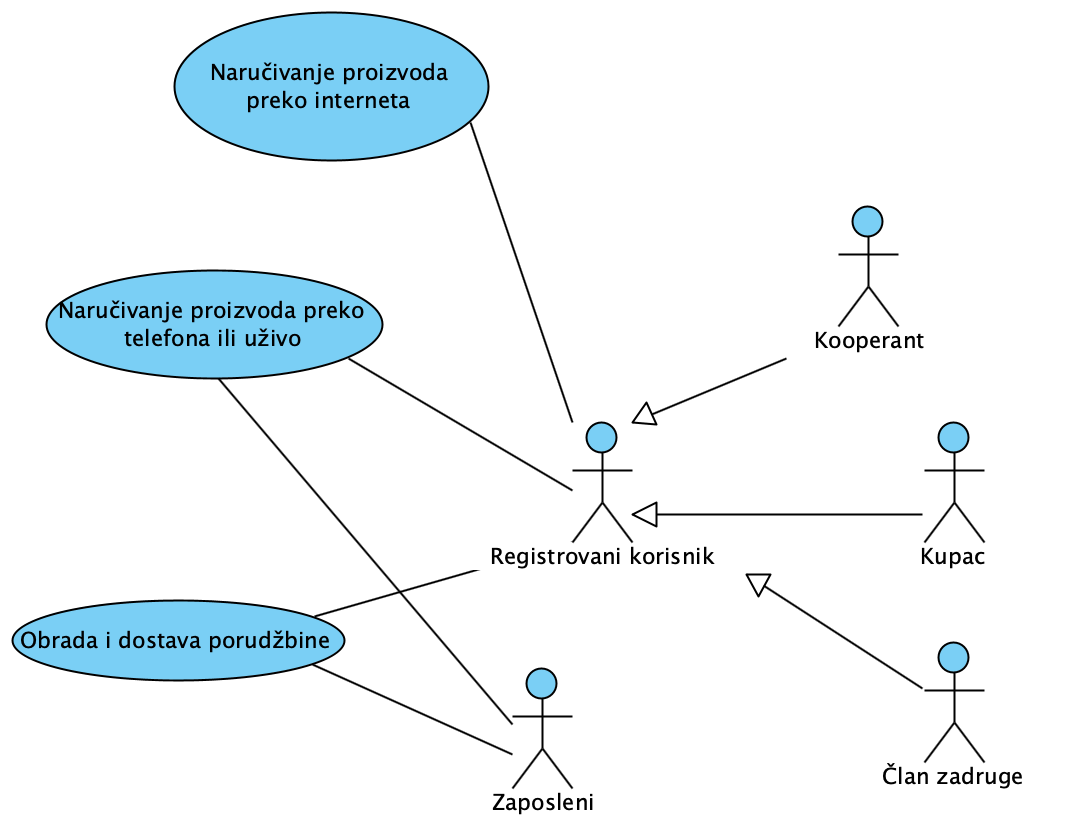
\includegraphics[scale=0.64]{images/dslucup_kupovina.png}
    \caption{Dijagram slučaja upotrebe vezanog za kupovinu}
    \label{dslucup_kupovina}
\end{figure}

\clearpage

\subsubsection{Naručivanje proizvoda preko interneta}
\begin{usecase}
        \addtitle{SLUČAJ UPOTREBE}{}
        \addfield{Naziv:}{Naručivanje proizvoda preko interneta}
        \addfield{Kratak opis:}{Registrovani korisnik želi da kupi proizvode preko sajta}
        \addfield{Učesnici:}{
            Registrovani korisnik
        }
        \addfield{Preduslovi:}{
           Korisnik je registrovan
        }
        \addfield{Postuslovi:}{
           Porudžbenica je uneta u sistem
        }

        \addscenario{Glavni tok:}{
            \item Korisnik odlazi na vebsajt i prijavljuje se
            \item Korisnik prelazi na sekciju proizvodi
            \item Korisnik bira željene proizvode i količinu i dodaje ih u korpu
            \item Korisnik proverava odabrane proizvode i njihovu količinu u svojoj korpi 
            \item Korisnik bira željeni način dostave i način plaćanja
            \item Sistem prikazuje korisniku ukupnu cenu izabranih proizvoda
            \item Korisnik potvrđuje porudžbinu
            \item Sistem obrađuje porudžbinu 
        }
        \addscenario{Alternativni tokovi:}{
            \item[4.a] Korisnik želi da naruči još neki proizvod. Slučaj upotrebe se nastavlja od koraka 3.
            \item[4.b] Korisnik je izbacio neki proizvod iz korpe. Slučaj upotrebe se nastavlja od koraka 4. 
            \item[7.a] Korisnik je poništio porudžbinom klikom na dugme za poništavanje. Slučaj upotrebe se završava.
        }
        \addfield{Dodatne informacije:}{
            Mogući načini dostave proizvoda su: 
            \begin{itemize}
                \item Lično preuzimanje u zadruzi (besplatno)
                \item Dostava od strane zadruge (jeftino, u zavisnosti od cene poručene robe može biti i besplatno, ali može potrajati do 7 dana)                
                \item Dostava po kurirskoj službi (skupo, ali zagarantovana isporuka u roku od 2 radna dana)
            \end{itemize}
            Mogući načini plaćanja proizvoda su: 
            \begin{itemize}
                \item Karticom
                \item Prilikom preuzimanja porudžbine  
            \end{itemize}
        }
\end{usecase}

\subsubsection{Naručivanje proizvoda preko telefona ili uživo}
\begin{usecase}
        \addtitle{SLUČAJ UPOTREBE}{}
        \addfield{Naziv:}{Naručivanje proizvoda preko telefona ili uživo}
        \addfield{Kratak opis:}{Registrovani korisnik želi da kupi proizvode putem poziva telefonskog broja zadruge ili odlaskom na adresu zadruge}
        \addfield{Učesnici:}{
            Registrovani korisnik, zaposleni zadruge
        }
        \addfield{Preduslovi:}{
           Korisnik je registrovan
        }
        \addfield{Postuslovi:}{
           Zaposleni unosi porudžbenicu u sistem
        }
        \addscenario{Glavni tok:}{
            \item Korisnik poziva ponuđeni na vebsajtu broj telefona zadruge ili odlazi na lokaciju zadruge koja je takođe ponuđena na vebsajtu    
            \item Zaposleni zahteva lične podatke korisnika radi identifikacije
            \item Korisnik obaveštava zaposlenog o svojim ličnim podacima 
            \item Korisnik obaveštava zaposlenog o proizvodima koje želi da poruči
            \item Zaposleni proverava dostupnost traženih proizvoda
            \item Korisnik bira željeni način dostave i način plaćanja
            \item Zaposleni obaveštava korisnika o ukupnoj ceni izabranih proizvoda
            \item Korisnik potvrđuje porudžbinu
            \item Zaposleni upisuje u sistem porudžbinu
        }
        \addscenario{Alternativni tokovi:}{
            \item[3.a] Korisnik nije registrovan u sistem zadruge, neophodno je da napravi nalog. Slučaj upotrebe se preusmerava na slučaj 'Registrovanje korisnika'.
            \item[7.a] Korisnik se predomislio u vezi kupovine. Slučaj upotrebe se nastavlja od koraka 4.
            \item[8.a] Korisnik je odustao od porudžbine. Slučaj upotrebe se završava.
        }
        \addfield{Dodatne informacije:}{
            Lični podaci koje zaposleni može da zahteva su:
            \begin{itemize}
                \item Korisničko ime, jmbg i email.
            \end{itemize}
        }
\end{usecase}


\subsubsection{Obrada i dostava porudžbine}

Na slici \ref{dsekv_obrada_dostava} je prikazan dijagram sekvence obrade i dostave porudžbine.
\begin{figure}[h!]
    \centering
    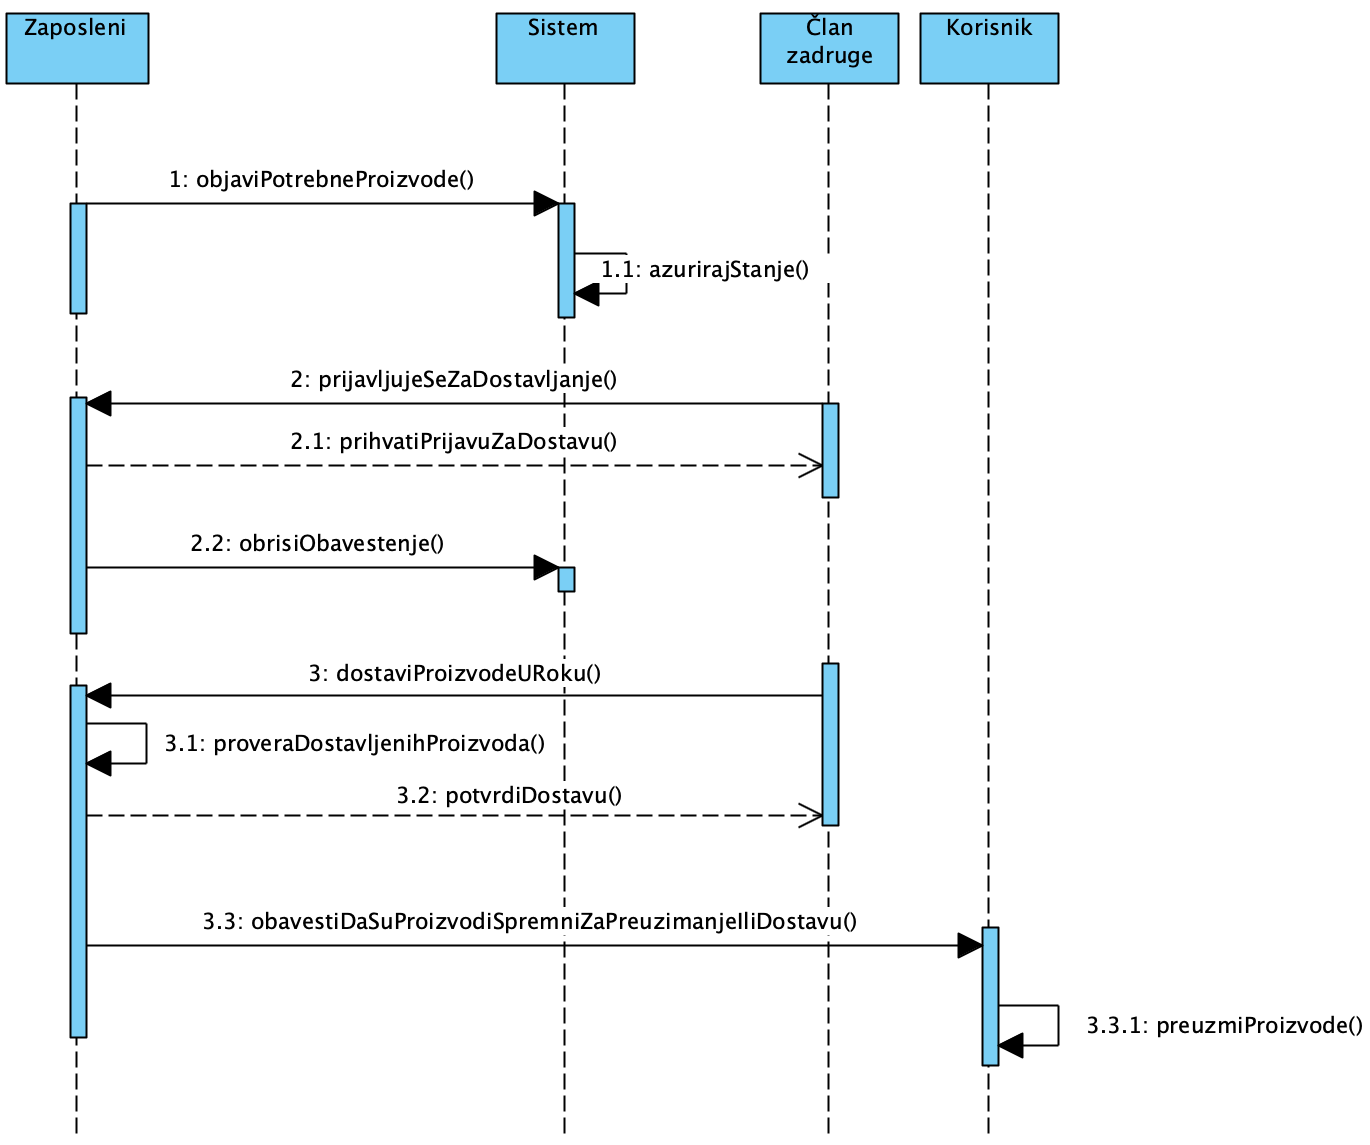
\includegraphics[scale=0.6]{images/dsekv_obrada_dostava.png}
    \caption{Dijagram sekvence obrade i dostave porudžbine}
    \label{dsekv_obrada_dostava}
\end{figure}
\clearpage

\begin{usecase}
        \addtitle{SLUČAJ UPOTREBE}{}
        \addfield{Naziv:}{Obrada porudžbine}
        \addfield{Kratak opis:}{Obrada porudžbine i organizacija dostave}
        \addfield{Učesnici:}{
            Zaposleni, član zadruge, registrovani korisnik
        }
        \addfield{Preduslovi:}{
           Korisnik je naručio proizvode iz zadruge
        }
        \addfield{Postuslovi:}{
           Korisnik je preuzeo poručene proizvode
        }
        \addscenario{Glavni tok:}{
            \item Zaposleni objavljuje na vebsajtu obaveštenje o proizvodima i njihovoj količini koji trebaju biti dostavljeni u zadrugu
            \item Član zadruge se javlja zaposlenom putem poziva da izvrši dostavu svih traženih proizvoda zadruzi 
            \item Zaposleni uklanja obaveštenje sa sajta
            
            \item Član zadruge dostavlja proizvode u zadrugu u datom roku
            \item Zaposleni proverava da li je dostavljeno sve što je i poručeno
            \item Korisnik je obavešten da se proizvodi koje je poručio nalaze u zadruzi i dat mu je rok od nedelju dana da iste preuzme na adresi zadruge
            \item Korisnik je preuzeo proizvode
            
        }  
        \addscenario{Alternativni tokovi:}{
             \item[2.a] Član zadruge je odgovorio da će dostaviti deo proizvoda u zadrugu. Obaveštenje se automatski ažurira. Slučaj upotrebe se nastavlja od koraka 1.
             \item[6.a] Kurirska služba dostavlja proizvode na adresu kupca. Slučaj upotrebe se nastavlja od koraka 7.
             \item[6.b] Član zadruge dostavlja proizvode na adresu kupca. Slučaj upotrebe se nastavlja od koraka 7.
             \item[7.a] Korisnik nije primio porudžbinu u datom roku i proizvodi su vraćeni zadruzi, a zatim vlasnicima. Slučaj upotrebe se završava.
        }
        
\end{usecase}


\subsection{Ostalo}
Na slici %\ref{dtp_ostalo} je prikazan dijagram toka podataka za slučaj ostalo, , dok je na slici 
\ref{dslucup_ostalo} je prikazan dijagram slučajeva upotrebe ostalo.

%\begin{figure}[h!]
%    \centering
%    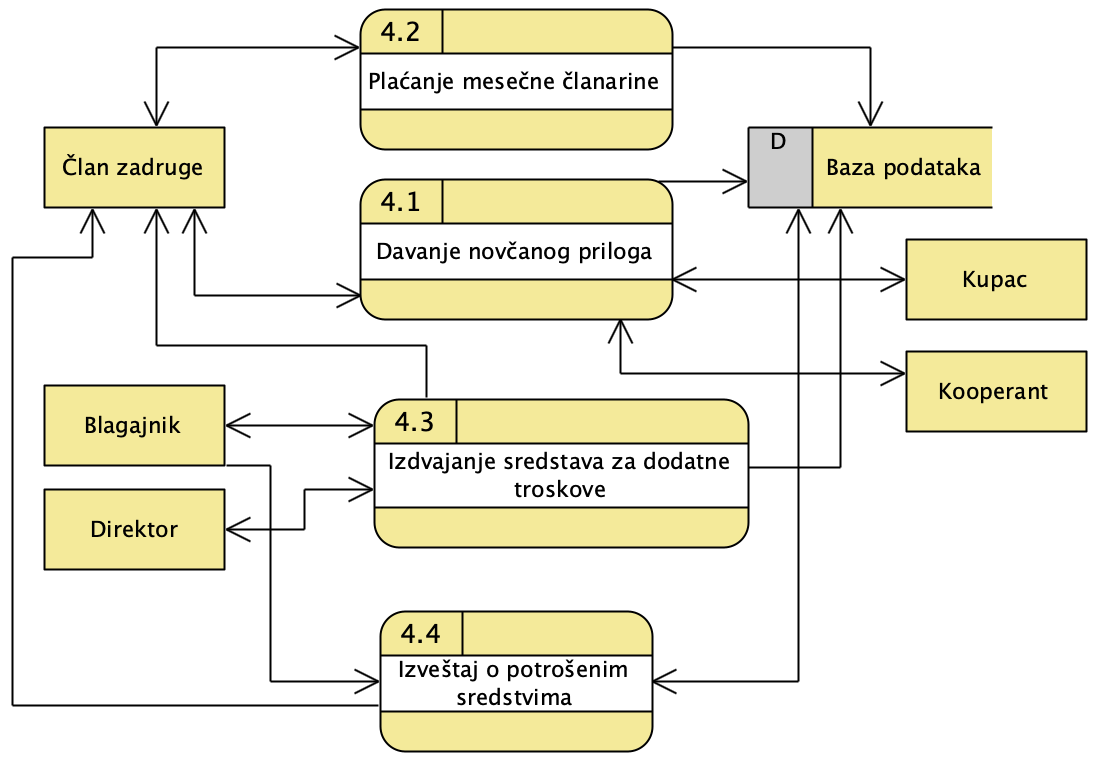
\includegraphics[scale=0.64]{images/dtp_ostalo.png}
%    \caption{Dijagram toka podataka za slučaj ostalo}
%    \label{dtp_ostalo}
%\end{figure}

\begin{figure}[h!]
    \centering
    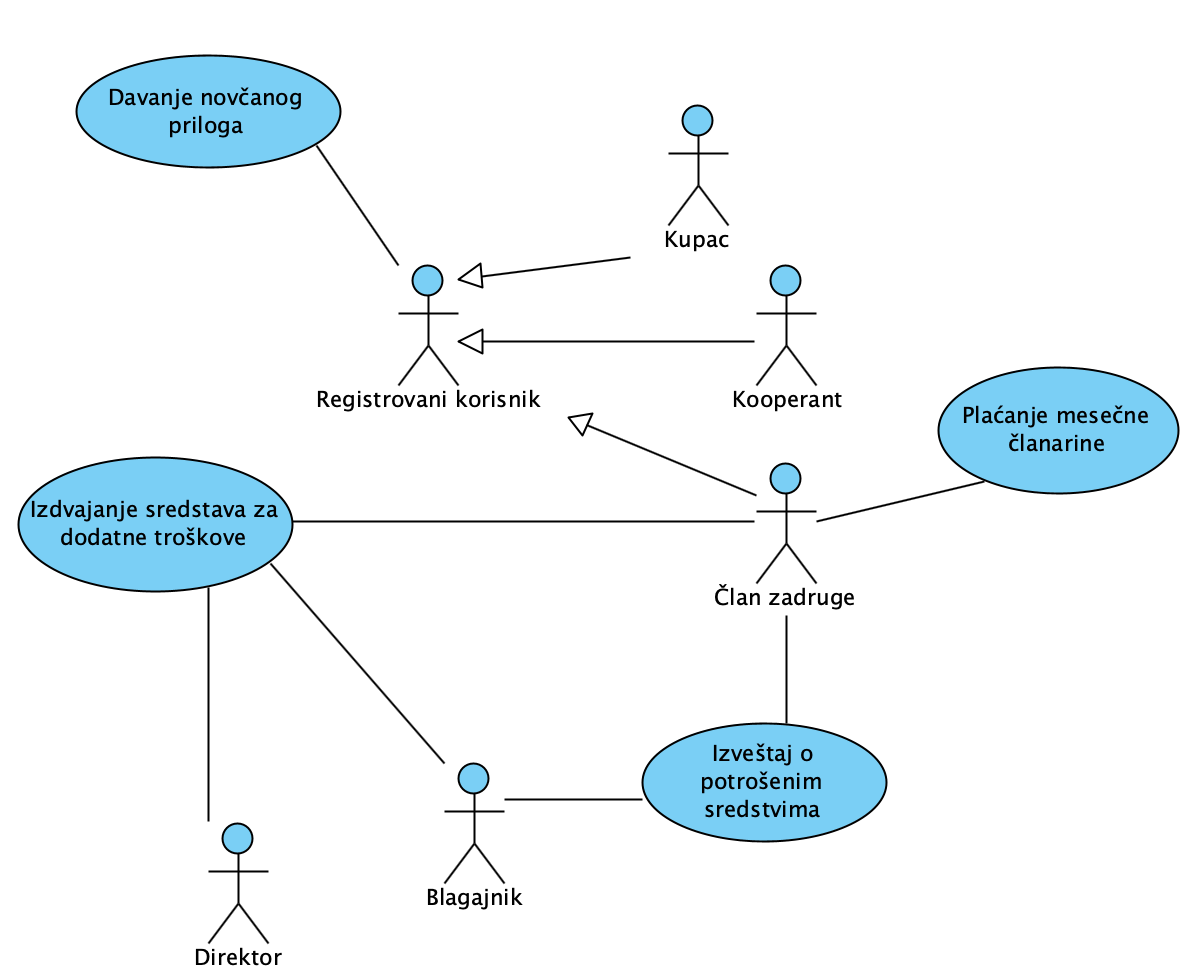
\includegraphics[scale=0.64]{images/dslucup_ostalo.png}
    \caption{Dijagram slučaja upotrebe vezanog za ostalo}
    \label{dslucup_ostalo}
\end{figure}

\clearpage

\subsubsection{Davanje novčanog priloga}
\begin{usecase}
        \addtitle{SLUČAJ UPOTREBE}{}
        \addfield{Naziv:}{Davanje priloga}
        \addfield{Kratak opis:}{Registrovani korisnik želi da donira novac zadruzi}
        \addfield{Učesnici:}{
            Registrovani korisnik (član zadruge/kooperant/kupac)
        }
        \addfield{Preduslovi:}{
           Korisnik je registrovan u sistemu
        }
        \addfield{Postuslovi:}{
           Korisnik je izvršio novčanu donaciju ukoliko je sistem adekvatno obradio podatke
        }

        \addscenario{Glavni tok:}{
            \item Korisnik odlazi na vebsajt i prijavljuje se
            \item Korisnik prelazi na formu za doniranje novca
            \item Korisnik unosi količinu novca i svrhu donacije
            \item Korisnik potvrđuje unesene podatke 
            \item Korisnik šalje zahtev sistemu
            \item Sistem obrađuje zahtev
            \item Sistem ažurira stanje na računu
            \item Korisnik dobija potvrdu o uplati
        }         
        \addscenario{Alternativni tokovi:}{
            \item[4.a]  Ukoliko korisnik nije uneo količinu novca, svrhu ili je uneo pogrešan format, prikazuje se odgovarajuča poruka. Slučaj upotrebe se nastavlja od koraka 2.
            \item[6.a] Ukoliko uplata nije prošla, korisnik dobija opciju da se vrati na korak 2, inače slučaj upotrebe se završava.
        }
\end{usecase}
\subsubsection{Plaćanje mesečne članarine}
Na slici \ref{bpmn_mesecna_clanarina} je prikazan BPMN dijagram plaćanja članarine.
\begin{figure}[h!]
    \centering
    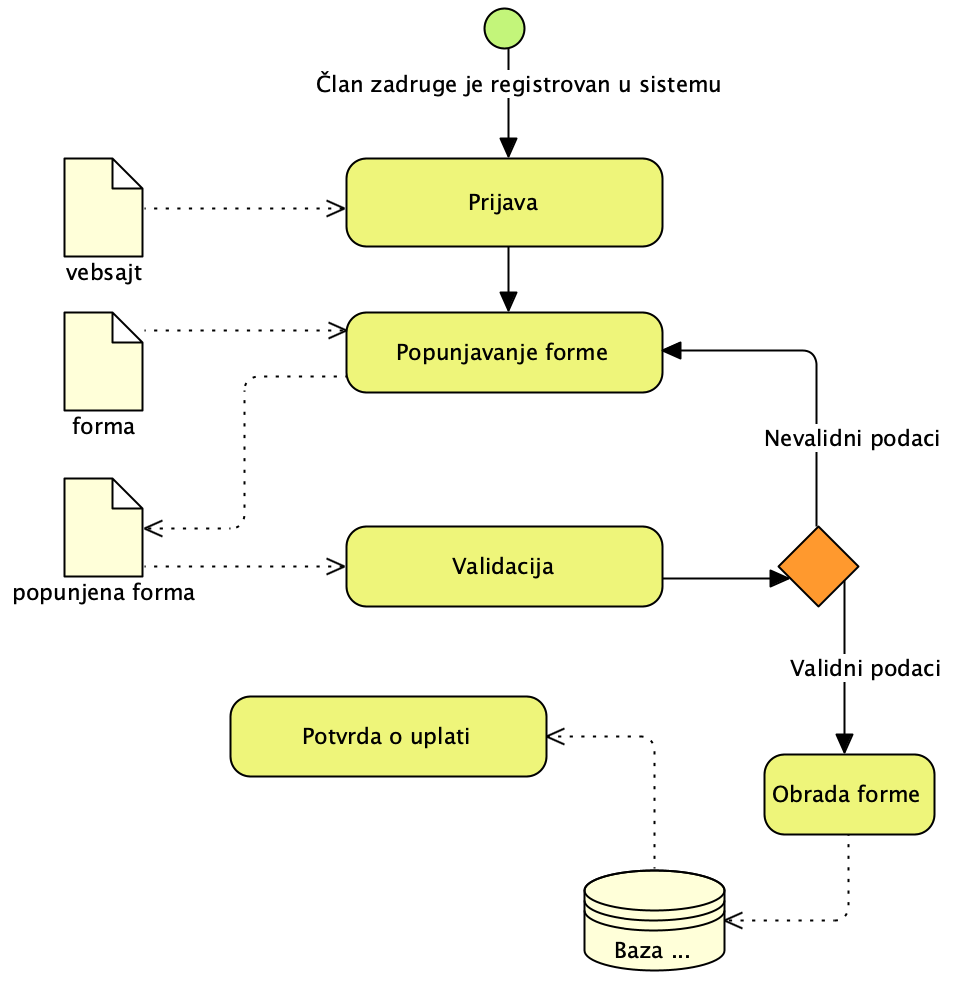
\includegraphics[scale=0.64]{images/bpmn_mesecna_clanarina.png}
    \caption{BPMN dijagram plaćanja članarine}
    \label{bpmn_mesecna_clanarina}
\end{figure}
\clearpage

\begin{usecase}
        \addtitle{SLUČAJ UPOTREBE}{}
        \addfield{Naziv:}{Plaćanje mesečne članarine}
        \addfield{Kratak opis:}{Član zadruge želi da uplati mesečnu članarinu}
        \addfield{Učesnici:}{
            Član zadruge
        }
        \addfield{Preduslovi:}{
           Član zadruge je registrovan u sistemu
        }
        \addfield{Postuslovi:}{
           Član zadruge je platio članarinu ukoliko je sistem adekvatno obradio podatke
        }

        %Main Success Scenario: A typical, unconditional happy path scenario of success.
        \addscenario{Glavni tok:}{
            \item Korisnik odlazi na vebsajt i prijavljuje se
            \item Korisnik prelazi na formu za uplatu članarine
            \item Korisnik unosi vrednost članarine
            \item Korisnik potvrđuje unesene podatke
            \item Korisnik šalje zahtev sistemu
            \item Sistem obrađuje zahtev
            \item Sistem ažurira korisnikova zaduženja
            \item Korisnik dobija potvrdu o uplati
        }
        \addscenario{Alternativni tokovi:}{
            \item[4.a] Ukoliko korisnik nije uneo količinu novca, svrhu ili je uneo pogrešan format, prikazuje se odgovarajuča poruka. Slučaj upotrebe se nastavlja od koraka 2.
            \item[6.a] Ukoliko uplata nije prošla, korisnik dobija opciju da se vrati na korak 2, inače slučaj upotrebe se završava.
        }
\end{usecase}

\subsubsection{Izdvajanje sredstava za dodatne troškove}
\begin{usecase}
        \addtitle{SLUČAJ UPOTREBE}{}
        \addfield{Naziv:}{Izdvajanje sredstava za dodatne troškove}
        \addfield{Kratak opis:}{Direktor zahteva novac od blagajnika za pokrivanje dodatnih troškova i obaveštava članove zadruge}
        \addfield{Učesnici:}{
            Direktor,
            blagajnik,
            član zadruge
        }
        \addfield{Preduslovi:}{
           Stanje na računu zadruge je pozitivno
        }
        \addfield{Postuslovi:}{
           Stanje na računu zadruge je pozitivno
        }

        \addscenario{Glavni tok:}{
            \item Direktor zadruge odlazi na vebsajt i prijavljuje se
            \item Direktor prelazi na formu za stvaranje dodatnog troška
            \item Direktor unosi razlog i potrebnu količinu novca za pokrivanje troškova
            \item Direktor potvrđuje unesene podatke
            \item Direktor šalje zahtev blagajniku
            \item Blagajnik proverava zahtev direktora
            \item Blagajnik obaveštava direktora o statusu zahteva
            \item Blagajnik odvaja novac za dodatni trošak
            \item Blagajnik obaveštava direktora da je novac izdvojen
            \item Direktor obaveštava članove zadruge o dodatnim troškovima
        }
        \addscenario{Alternativni tokovi:}{
            \item[4.a] Ukoliko direktor nije uneo razlog za pokrivanje troškova, prikazuje se odgovarajuća poruka. Slučaj upotrebe se nastavlja od koraka 2.
            \item[4.b] Ukoliko direktor nije uneo potrebnu količinu novca za pokrivanje troškova, prikazuje se odgovarajuća poruka. Slučaj upotrebe se nastavlja od koraka 2.
            \item[7.a] Ukoliko bi stanje na računu postalo negativno nakon izdvajanja novca, blagajnik obaveštava direktora da nije moguće trenutno izdvojiti potrebnu količinu novca za pokrivanje troškova. Slučaj upotrebe se završava.
            
        }
\end{usecase}
\subsubsection{Izveštaj o potrošenim sredstvima}
\begin{usecase}
        \addtitle{SLUČAJ UPOTREBE}{}
        \addfield{Naziv:}{Izveštaj o potrošenim sredstvima}
        \addfield{Kratak opis:}{Blagajnik izveštava članove zadruge o utrošenom novcu}
        \addfield{Učesnici:}{
            Blagajnik, članovi zadruge
        }
        \addfield{Preduslovi:}{
           Svi učesnici su registrovani
        }
        \addfield{Postuslovi:}{
           Svi učesnici su obavešteni o tekučem stanju na računu zadruge i utrošenim sredstvima
        }

        %Main Success Scenario: A typical, unconditional happy path scenario of success.
        \addscenario{Glavni tok:}{
            \item Blagajnik zadruge odlazi na vebsajt i prijavljuje se
            \item Blagajnik prelazi na formu za stvaranje mesečnog izveštaja
            \item Blagajnik popunjava formu
            \item Blagajnik potvrđuje unesene podatke
            \item Sistem obrađuje zahtev
            \item Sistem generiše izveštaj
            \item Sistem obaveštava sve učesnike o tekućem stanju na računu zadruge
        }
        \addscenario{Alternativni tokovi:}{
            \item[4.a] Ukoliko blagajnik nije popunio formu, prikazuje se odgovarajuća poruka. Slučaj upotrebe se nastavlja od koraka 2.
            
        }
        \addfield{Dodatne informacije:}{Forma za stvaranje izveštaja sadrži sledeća polja: datum od kojeg se traže prihodi i rashodi, format dokumenta (pdf/docx/csv), korisnici kojima se šalje izveštaj (direktor/članovi zadruge)}
\end{usecase}

\section{Predlog arhitekture sistema}

\begin{figure}[h!]
    \centering
    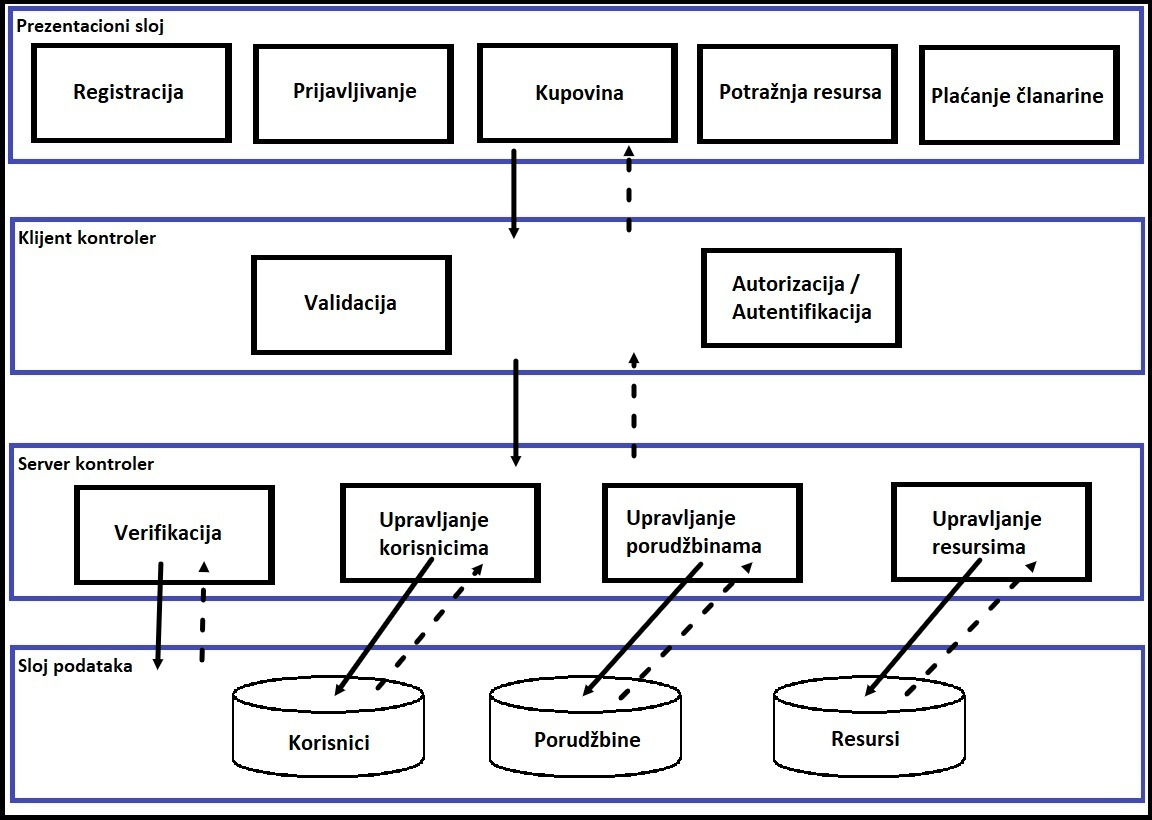
\includegraphics[scale=0.335]{images/Predlog_arhitekture.jpg}
    \caption{Predlog arhitekture sistema}
    \label{predlog_arhitekture_sistema}
\end{figure}

\subsection{Karakteristike}

\begin{enumerate}
    \item Tip aplikacije: veb aplikacija
    \item Strategija isporučivanja: jedan serverski i više klijentskih računara
    \item Odgovarajuće tehnologije: Java, MySQL, JavaFX, JS, HTML5, CSS3
\end{enumerate}

\indent Ovako organizovan sistem je jednostavan za održavanje, skalabilan je tj jednostavno se povećava broj klijenata, veb aplikacija omogućava visok stepen ažurnosti. Ukoliko bude potrebe mogu se uzeti dodatni serveri, čime bi se povećala fleksibilnost i pouzdanost sistema. Logika aplikacije se može menjati i u toku rada.

\subsection{Slojevi arhitekture}

\indent Veb aplikaciju predstavlja višeslojna klijent-server arhitektura, koja je prikazana na slici \ref{predlog_arhitekture_sistema}. Arhitekturu čine prezentacioni sloj, klijent kontroler, server kontroler i sloj podataka.

\subsubsection{Prezentacioni sloj}
Glavni zadatak prezentacionog sloja je da omogući korisniku komunikaciju sa sistemom, tako da ona bude što efikasnija i jednostavnija. Pruža sledeće mogućnosti:
\begin{itemize}
    \item Registracija
    \item Prijavljivanje
    \item Kupovina
    \item Potražnja resursa
    \item Plaćanje članarine
\end{itemize}

\subsubsection{Klijent kontroler}
Omogućava komunikaciju sa serverskim slojem sistema. Takođe, izvršava validaciju podataka kao i njihovu autorizaciju i autentifikaciju. Pruža sledeće mogućnosti:
\begin{itemize}
    \item Validacija
    \item Autorizacija / autentifikacija
\end{itemize}

\subsubsection{Server kontroler}
Ima sličnu ulogu kao klijent kontroler, s tim da klijent ne može pristupiti ovom sloju, pa se na njemu vrše dodatne provere podataka. Predstavlja posrednika u komunikaciji sa slojem podataka. Pruža sledeće mogućnosti:
\begin{itemize}
    \item Upravljanje korisnicima
    \item Upravljanje porudžbinama
    \item Upravljanje resursima
    \item Verifikacija
\end{itemize}

\subsubsection{Sloj podataka}
Sadrži bazu podataka i omogućuje bezbedan i lak pristup podacima. Shema baze podataka biće predstavljena u narednom delu \ref{baza_podataka}.

\section{Baza podataka}
\label{baza_podataka}

U ovom delu biće data shema predložene baze podataka sistema kao i opis entiteta koji se nalaze unutar sheme.

\subsubsection{Pregled entiteta}
Na slici \ref{predlog_baze_sistema} nalazi se shema predložene baze podataka. 
\begin{figure}[h!]
    \centering
    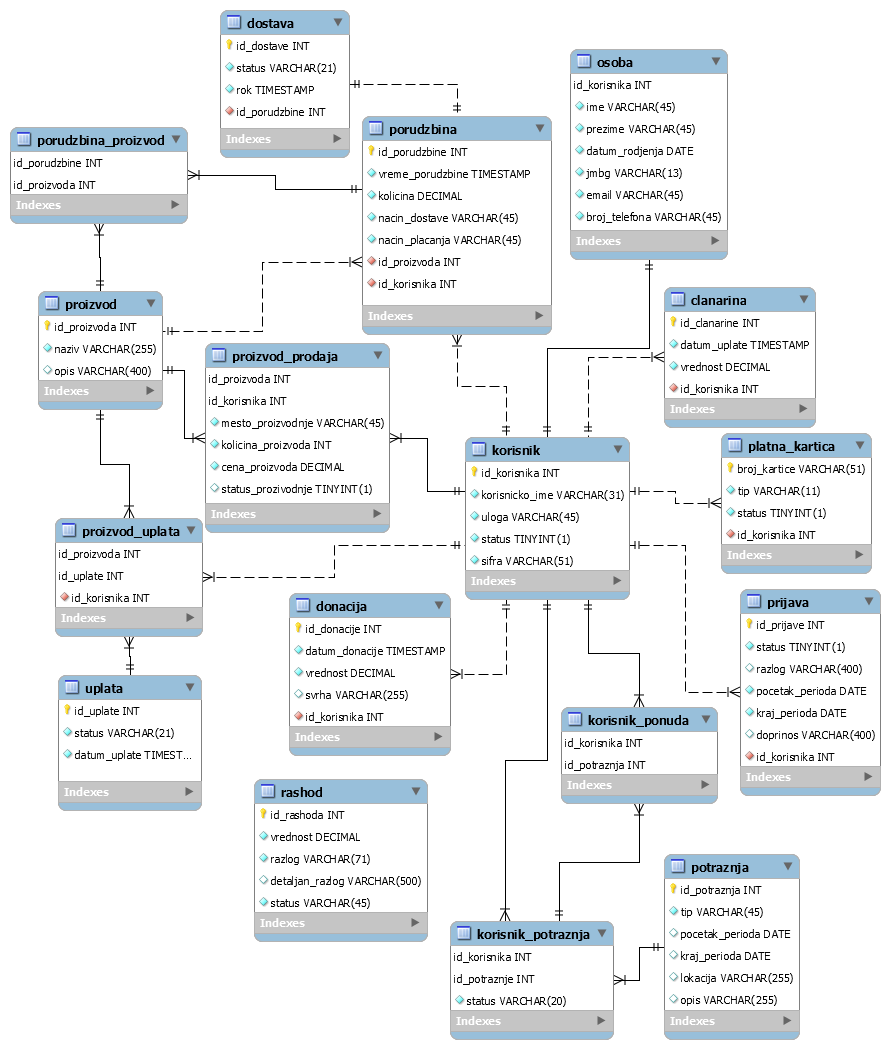
\includegraphics[scale=0.42]{images/baza.png}
    \caption{Shema baze podataka sistema}
    \label{predlog_baze_sistema}
\end{figure}

\subsubsection{Nezavisni entiteti}
Nezavisni entiteti u bazi podataka su
\begin{itemize}
    \item Korisnik
    \item Platna kartica
    \item Prijava
    \item Članarina
    \item Porudžbina
    \item Dostava
    \item Proizvod
    \item Donacija
    \item Rashod
    \item Potražnja
    \item Uplata
\end{itemize}
\subsubsection{Zavisni entiteti}
\begin{itemize}
    \item Osoba
\end{itemize}
\subsubsection{Agregirani entiteti}
\begin{itemize}
    \item Proizvod\_Prodaja
    \item Proizvod\_Uplata
    \item Porudžbina\_Proizvod
    \item Korisnik\_Potražnja
    \item Korisnik\_Ponuda
\end{itemize}

\section{Korisnički interfejs}
\label{korisnicki_interfejs}

\subsubsection{Početna strana}
\begin{figure}[h!]
    \centering
    
\includegraphics[scale=0.3]{images/home1.png}
    \caption{Početna strana - prvi slajd}
    \label{homepage1}
\end{figure}

\begin{figure}[h!]
    \centering
    \includegraphics[scale=0.3]{images/home2.png}
    \caption{Početna strana - drugi slajd}
    \label{homepage2}
\end{figure}

\newpage
\subsubsection{Sekcija o zadruzi}
\begin{figure}[h!]
    \centering
    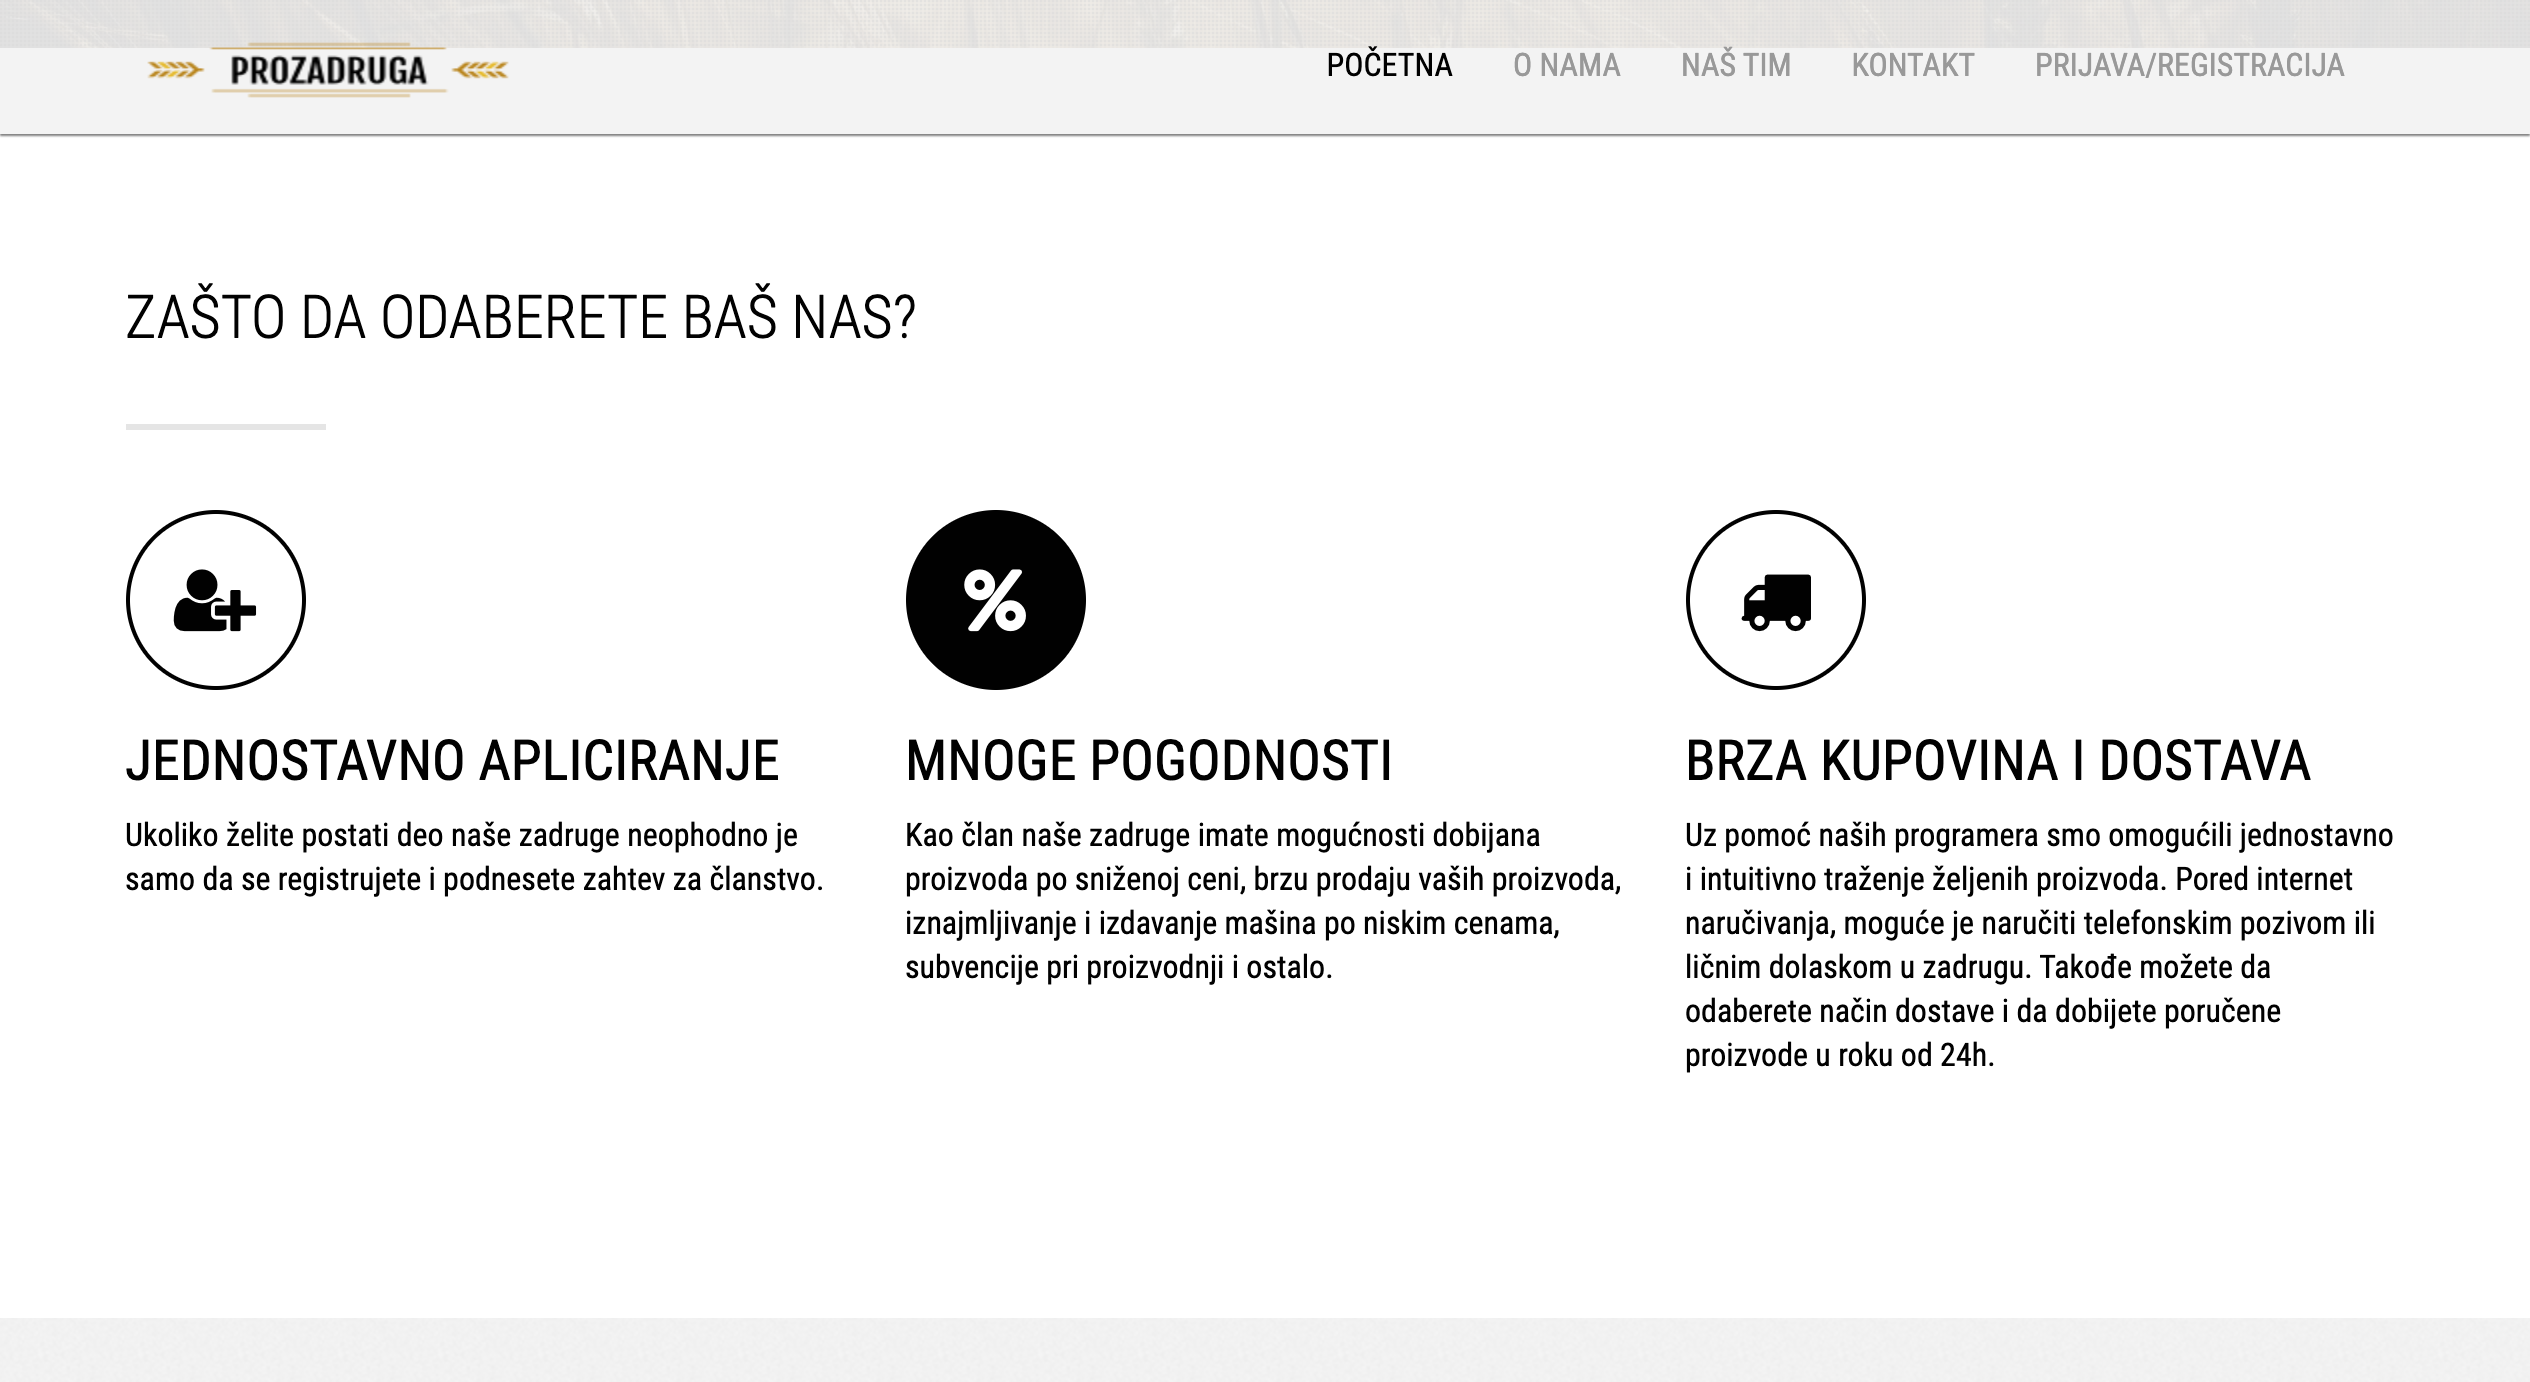
\includegraphics[scale=0.3]{images/about.png}
    \caption{O nama}
    \label{about}
\end{figure}

\begin{figure}[h!]
    \centering
    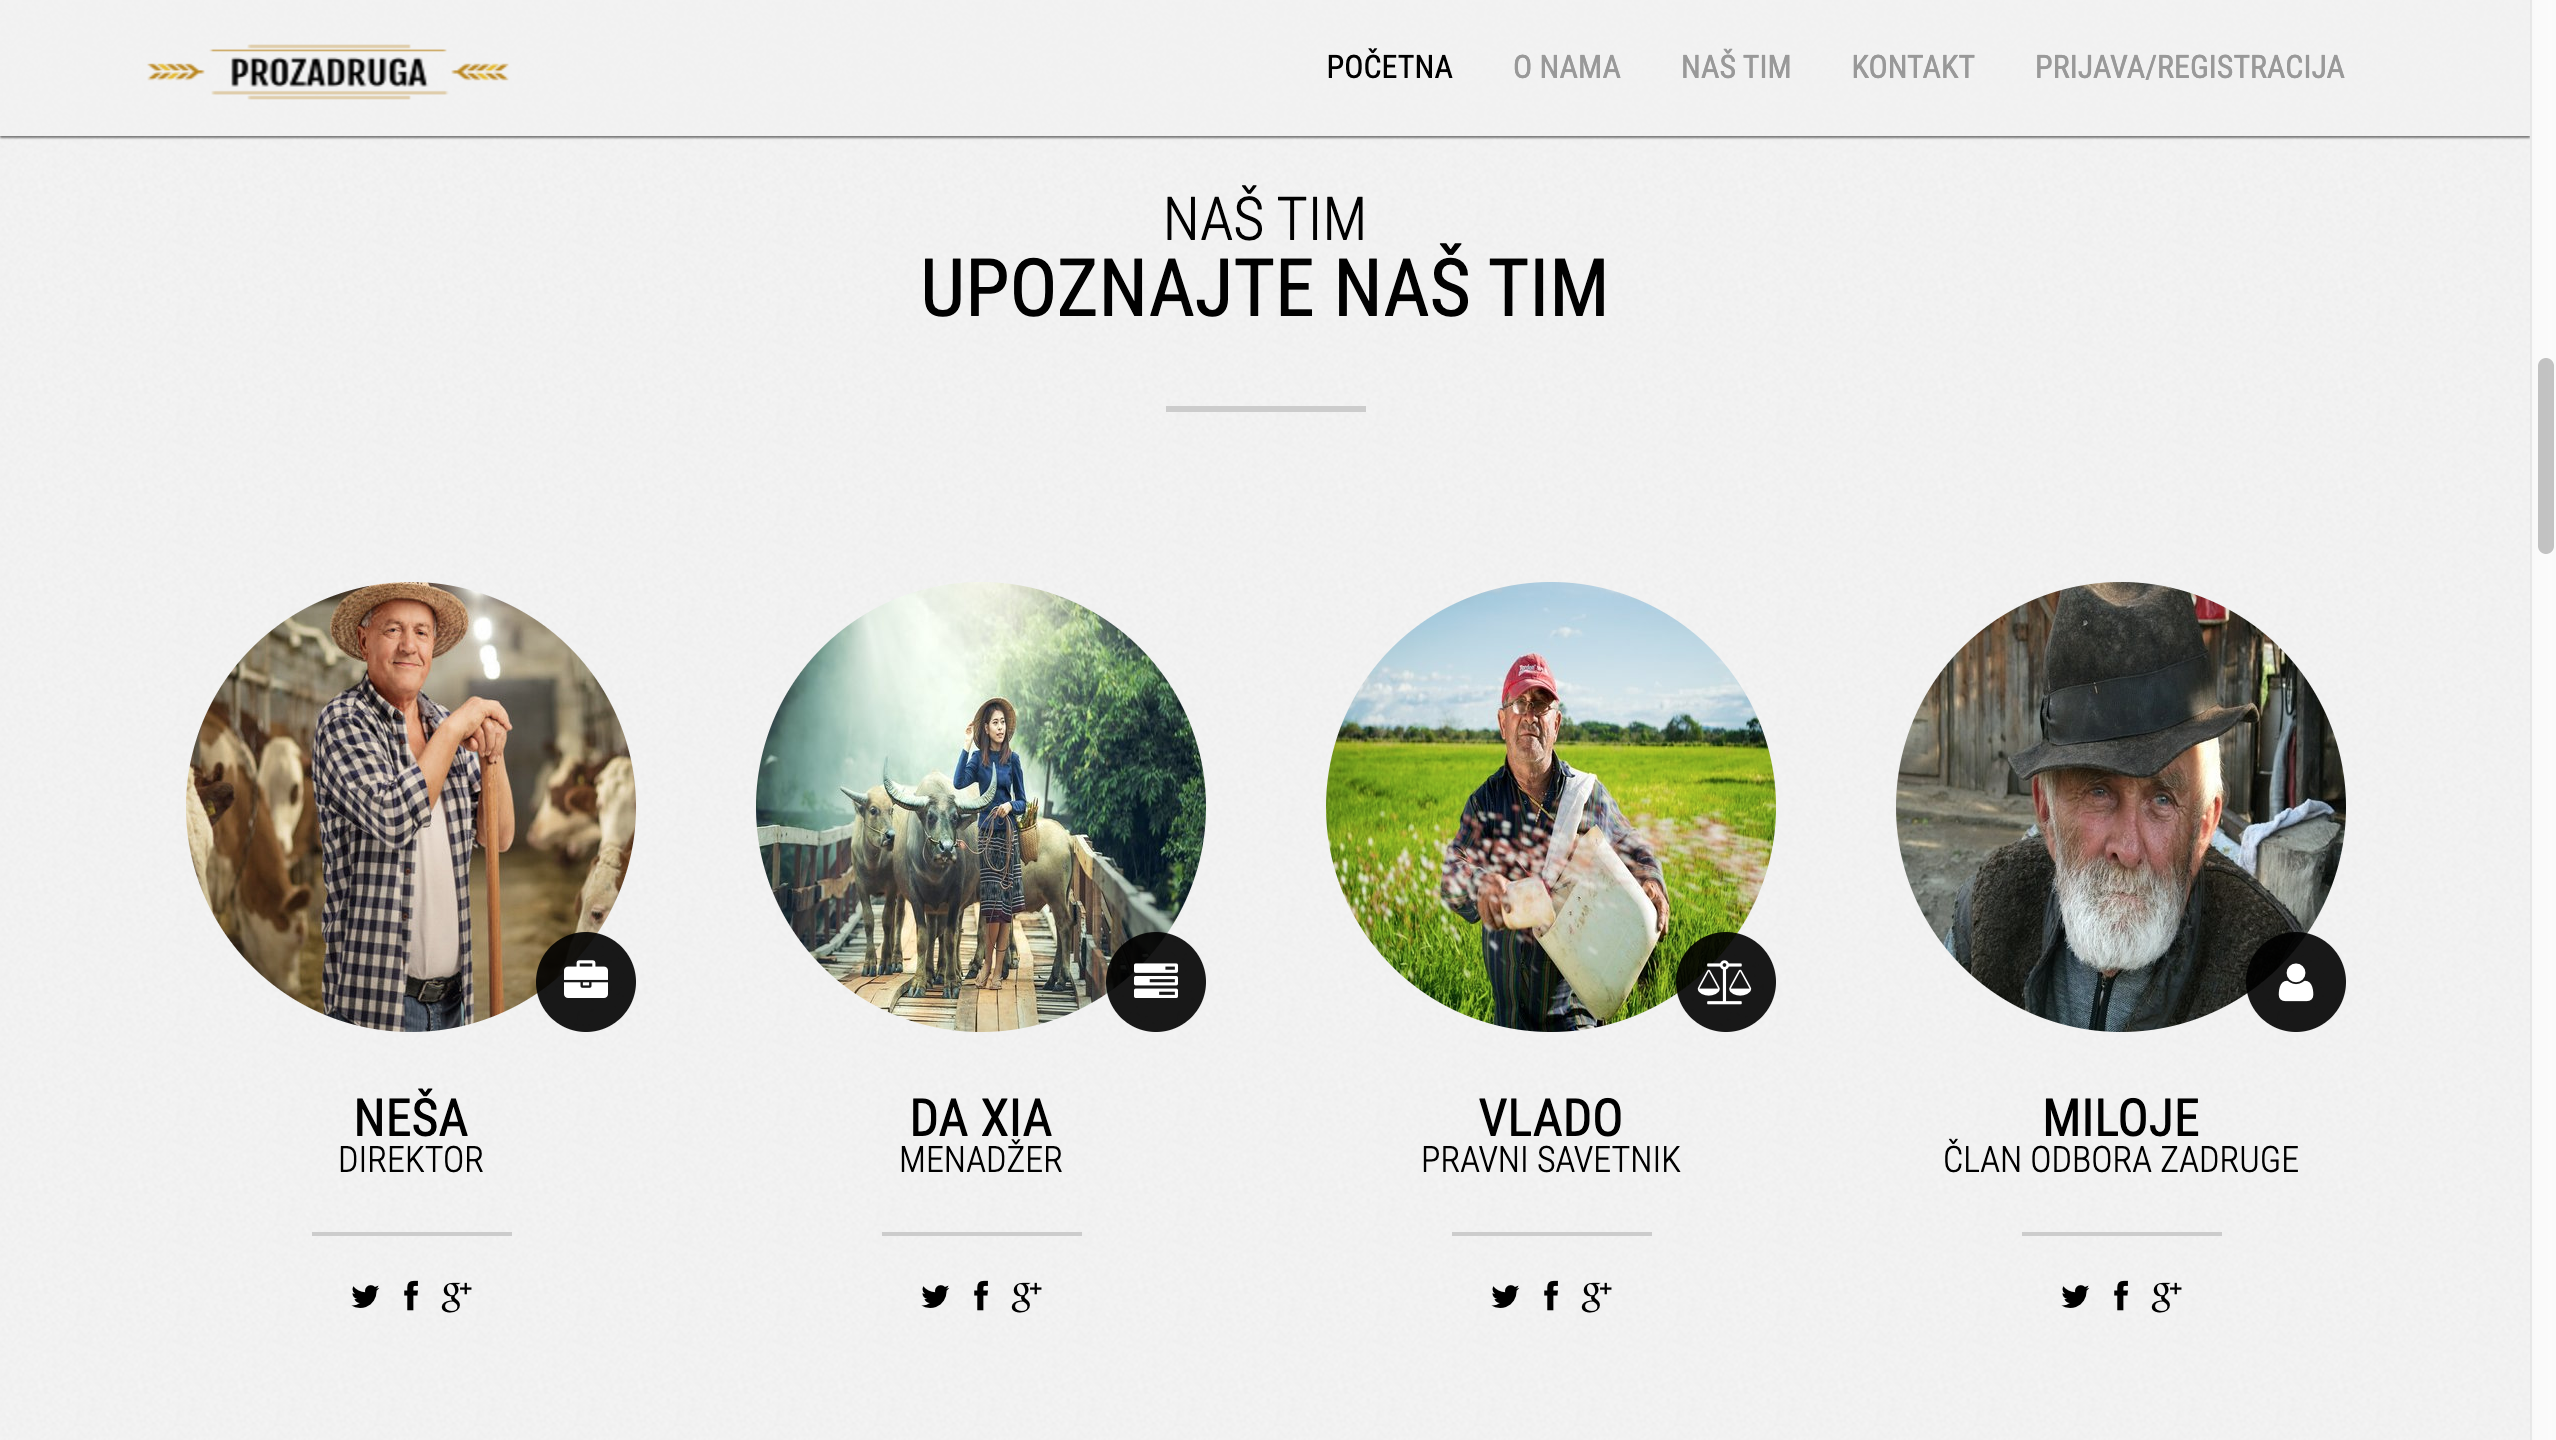
\includegraphics[scale=0.3]{images/team.png}
    \caption{Tim}
    \label{team}
\end{figure}

\newpage
\subsubsection{Prijavljivanje i registracija}
\begin{figure}[h!]
    \centering
    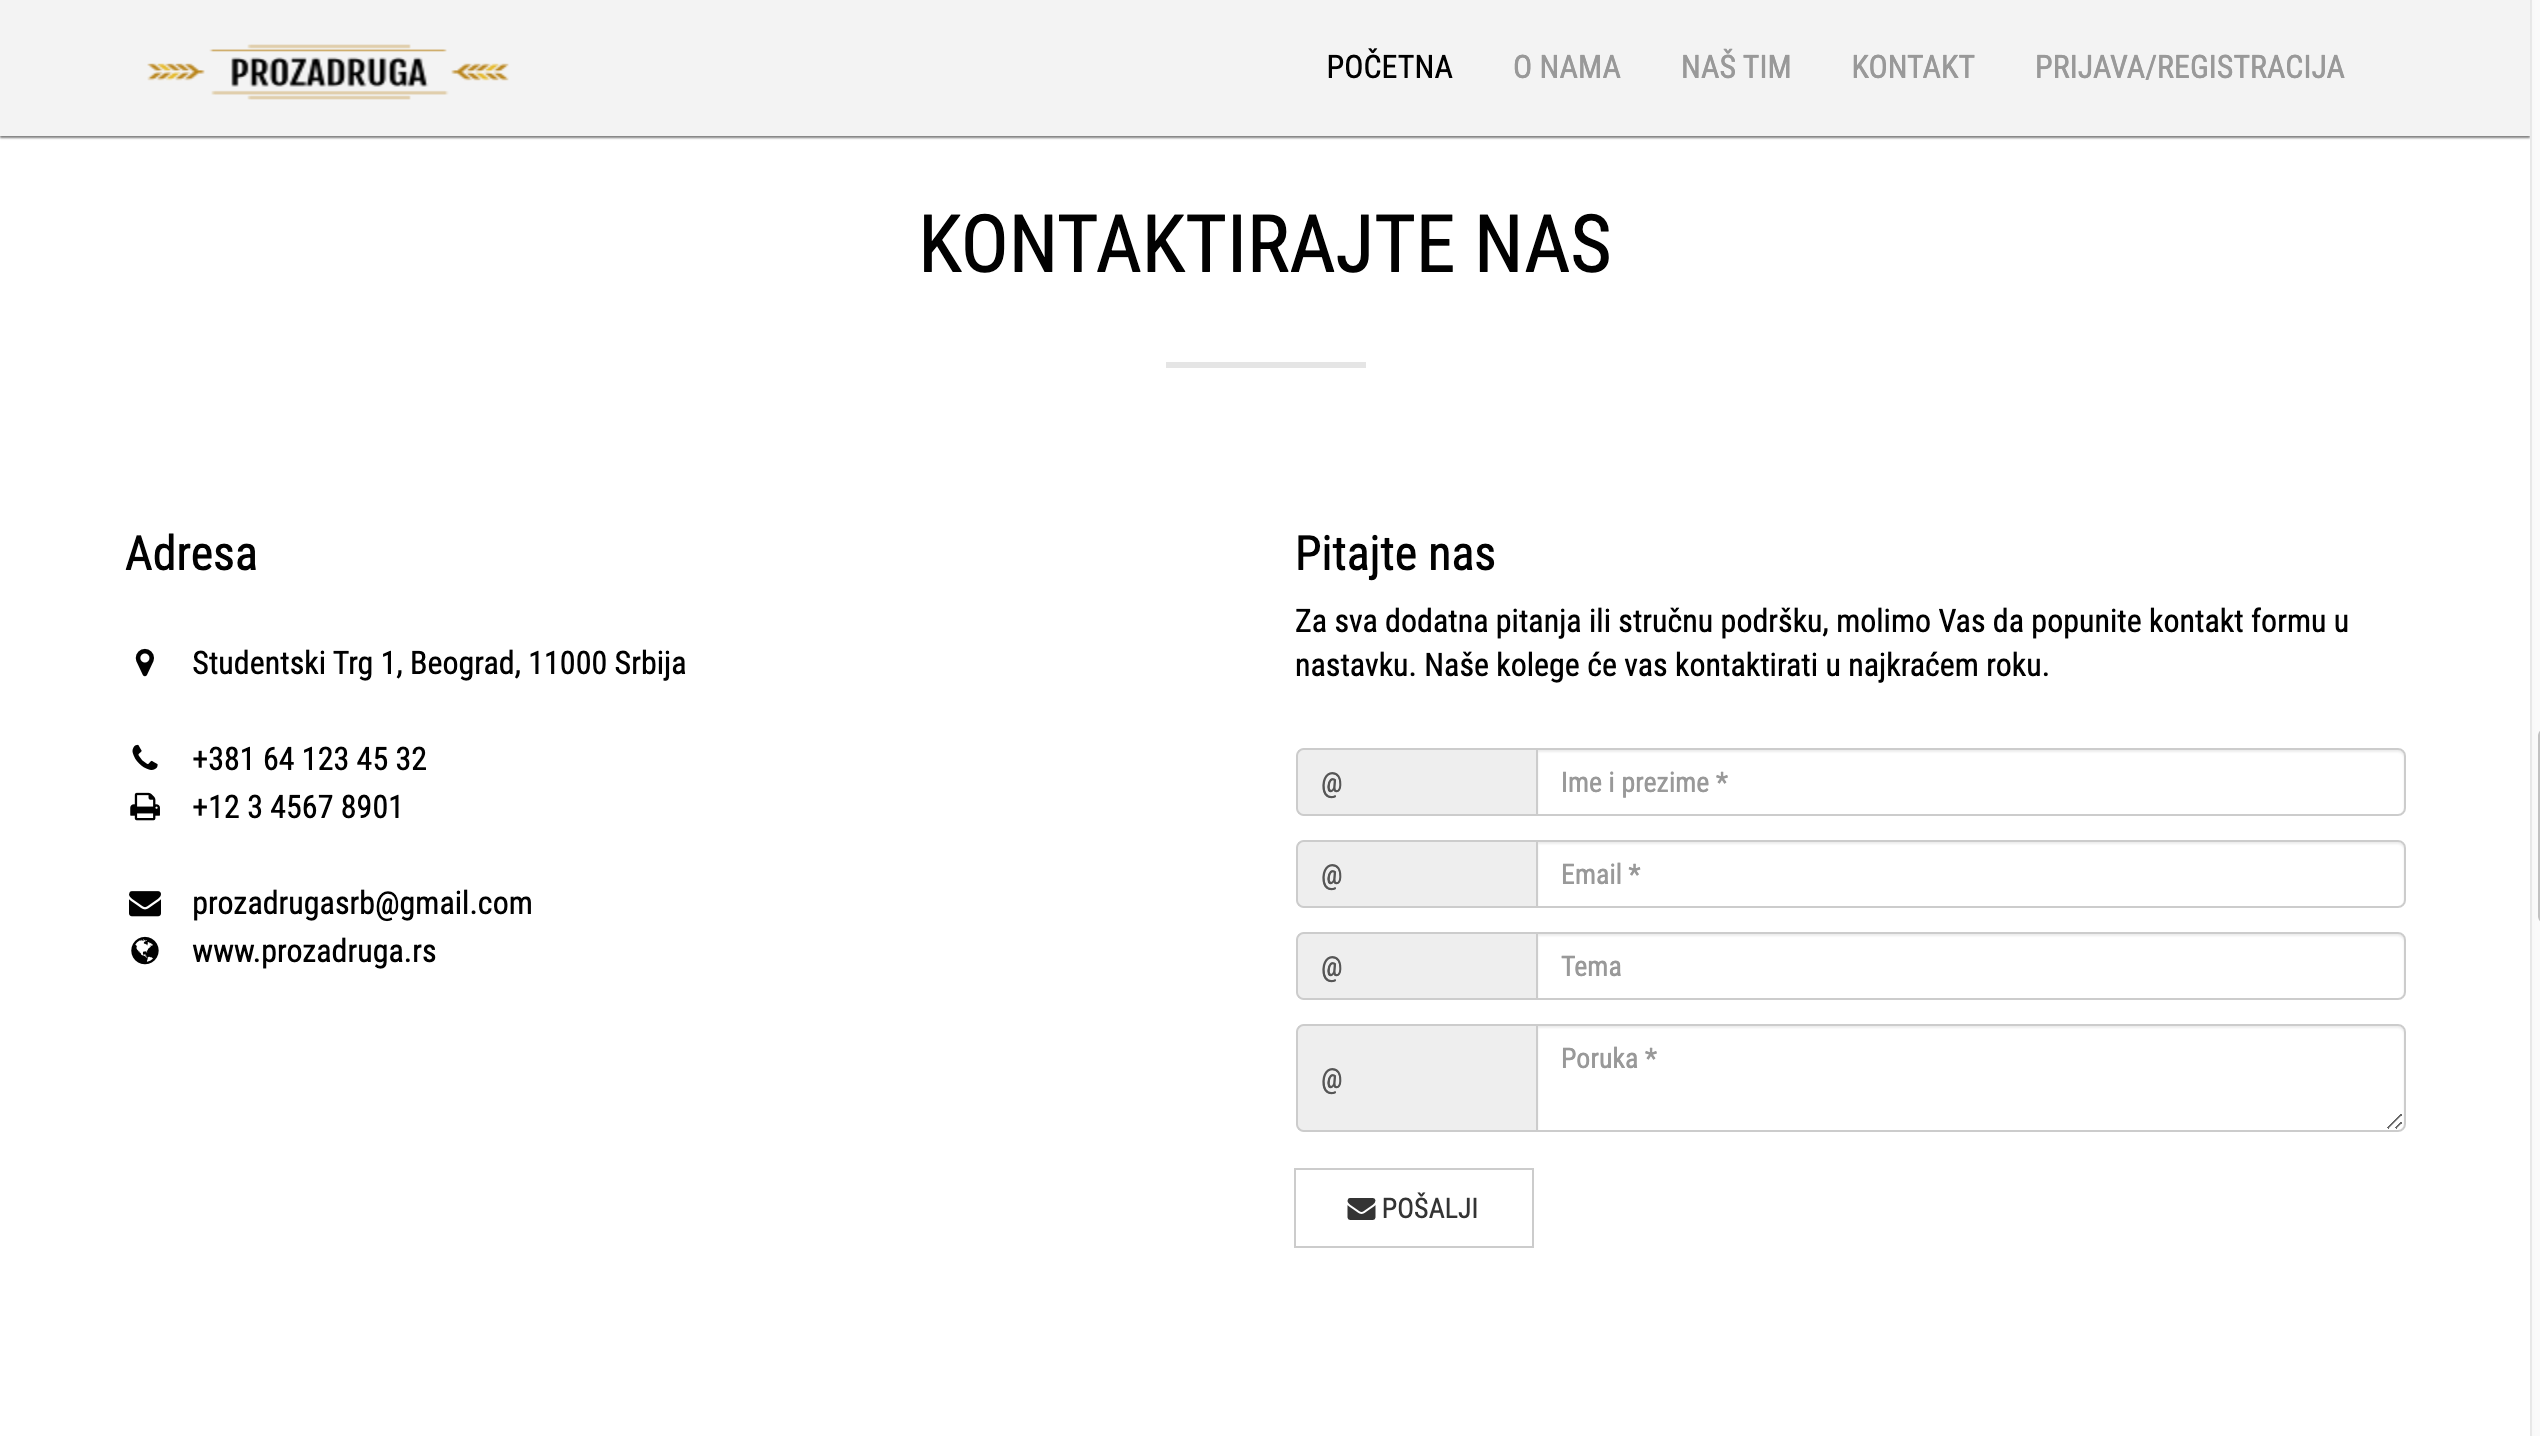
\includegraphics[scale=0.3]{images/contact.png}
    \caption{Kontakt}
    \label{contact}
\end{figure}

\begin{figure}[h!]
    \centering
    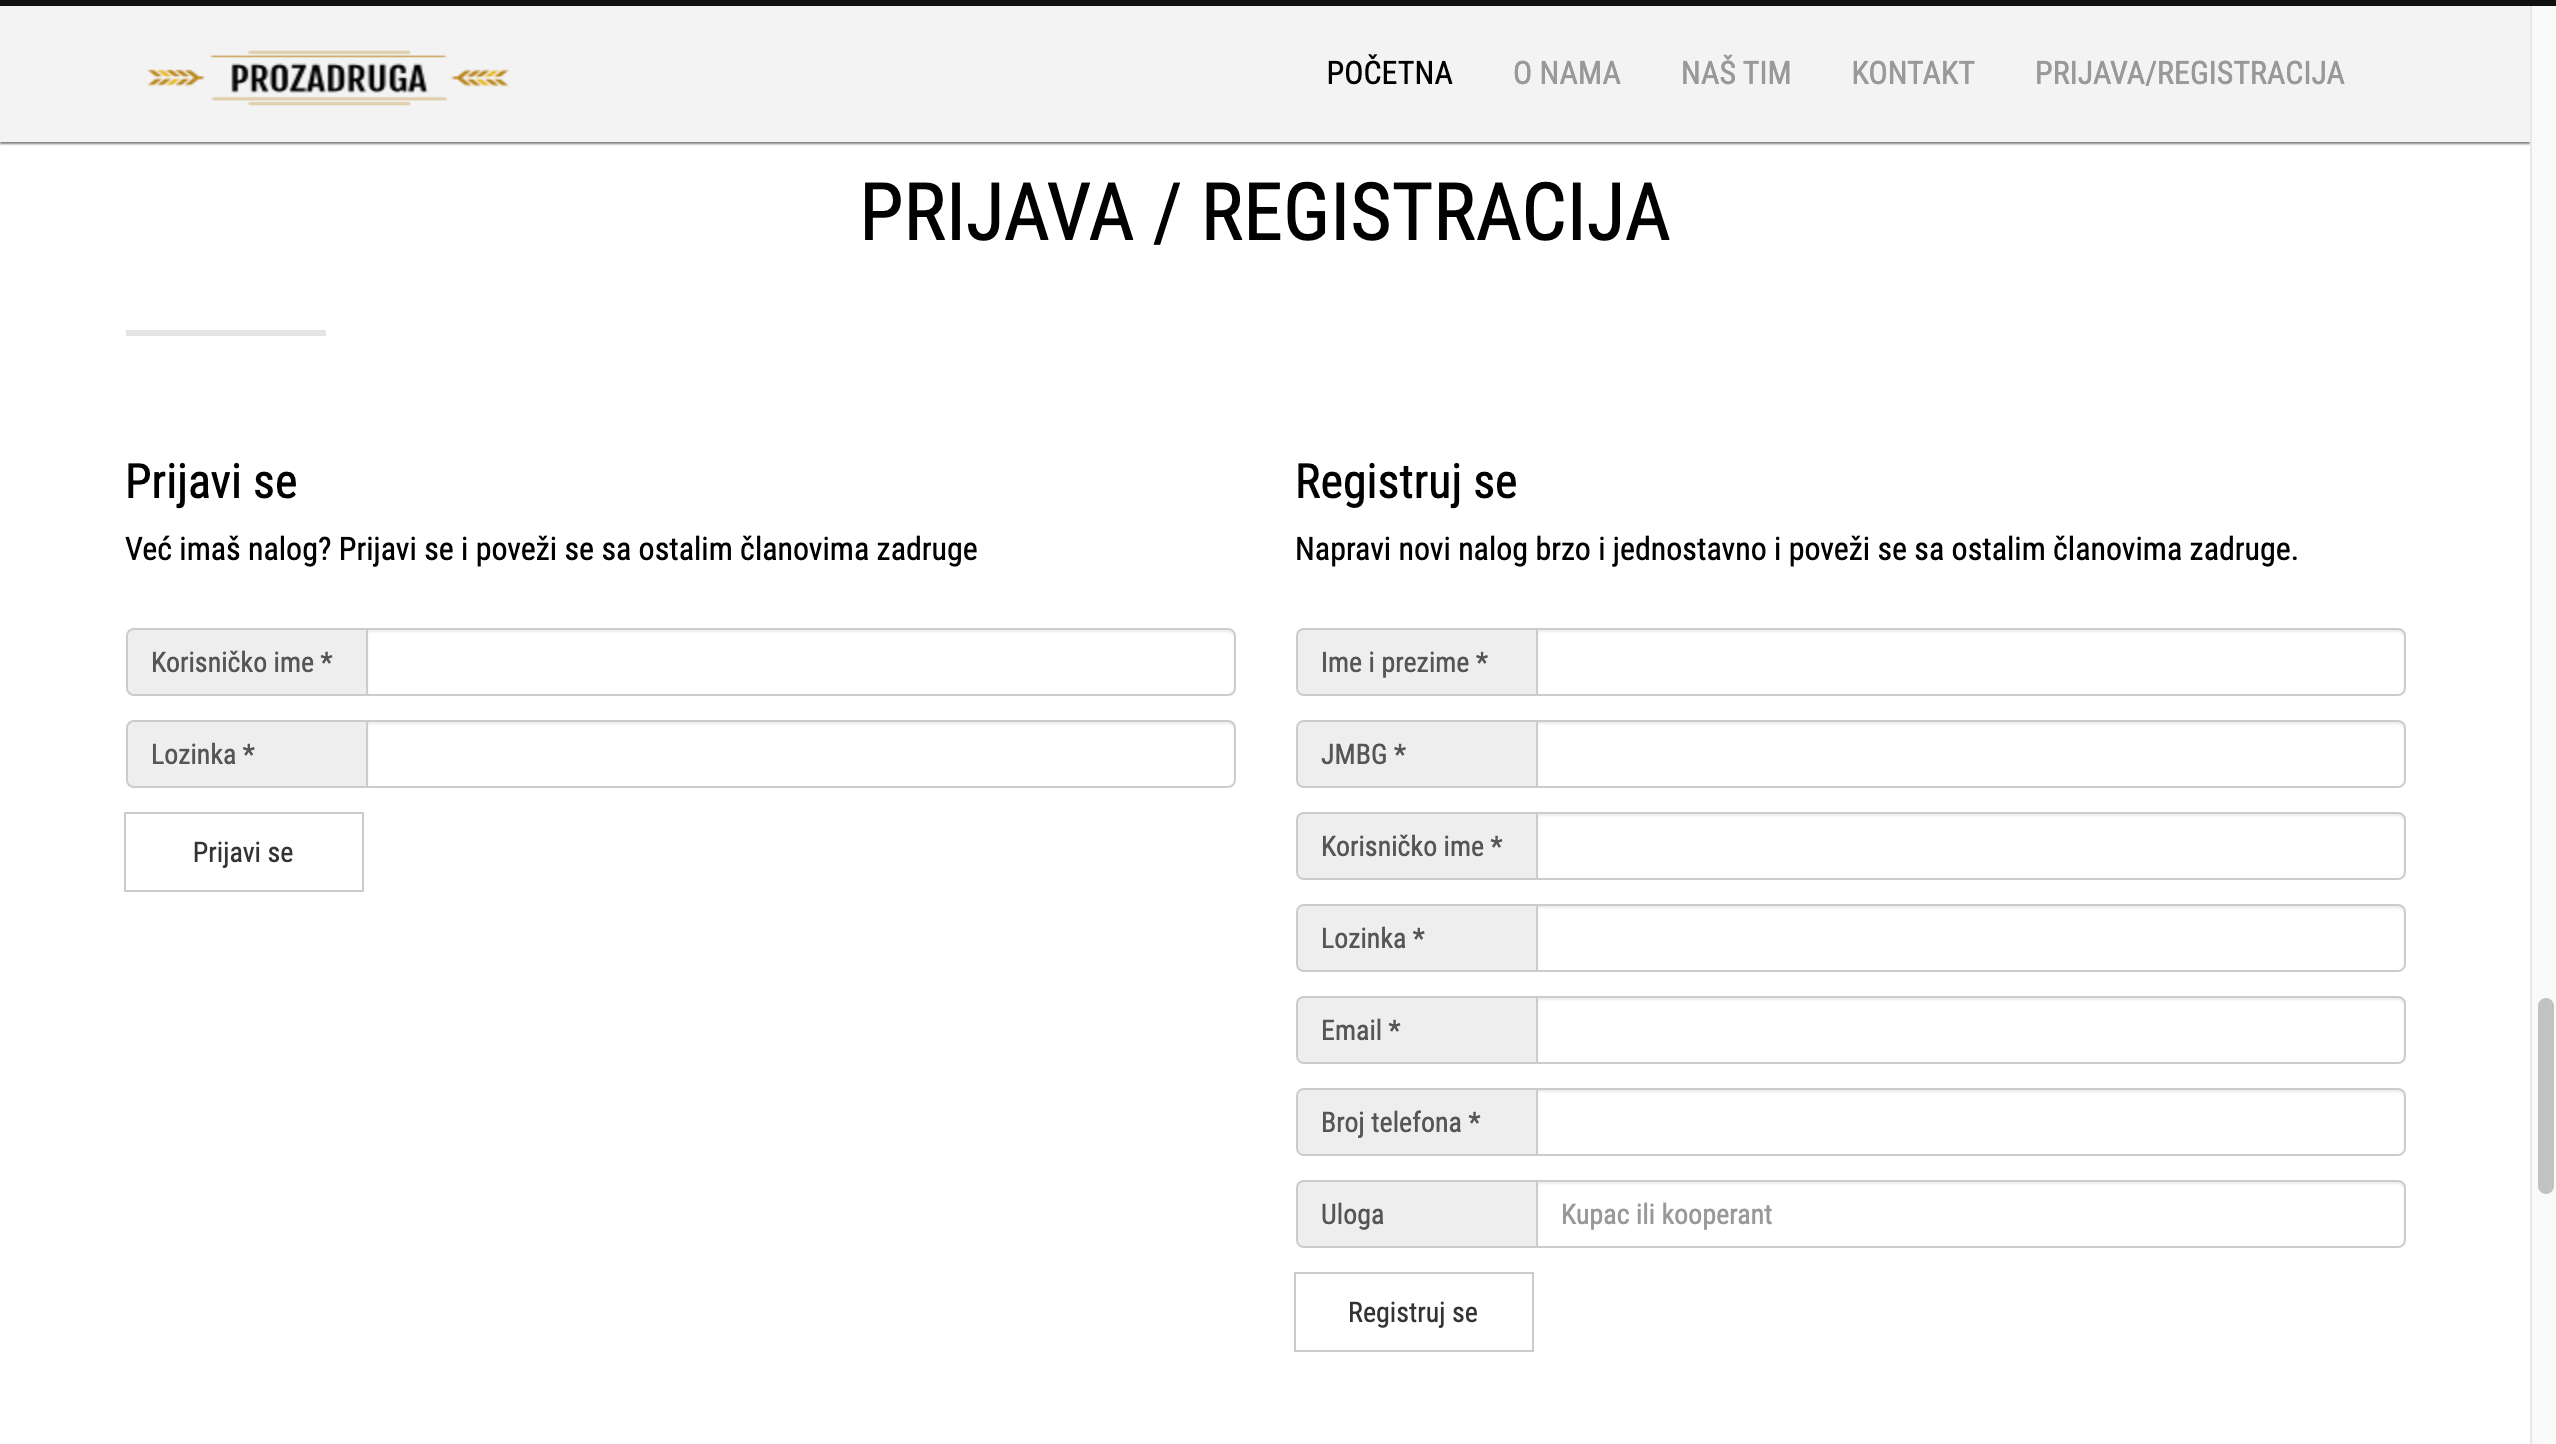
\includegraphics[scale=0.3]{images/register.png}
    \caption{Registracija i prijavljivanje}
    \label{register}
\end{figure}


\newpage
\subsubsection{Moj profil i potražnje}
\begin{figure}[h!]
    \centering
    
\includegraphics[scale=0.3]{images/profile1.png}
    \caption{Moj profil - početna strana}
    \label{profile1}
\end{figure}

\begin{figure}[h!]
    \centering
    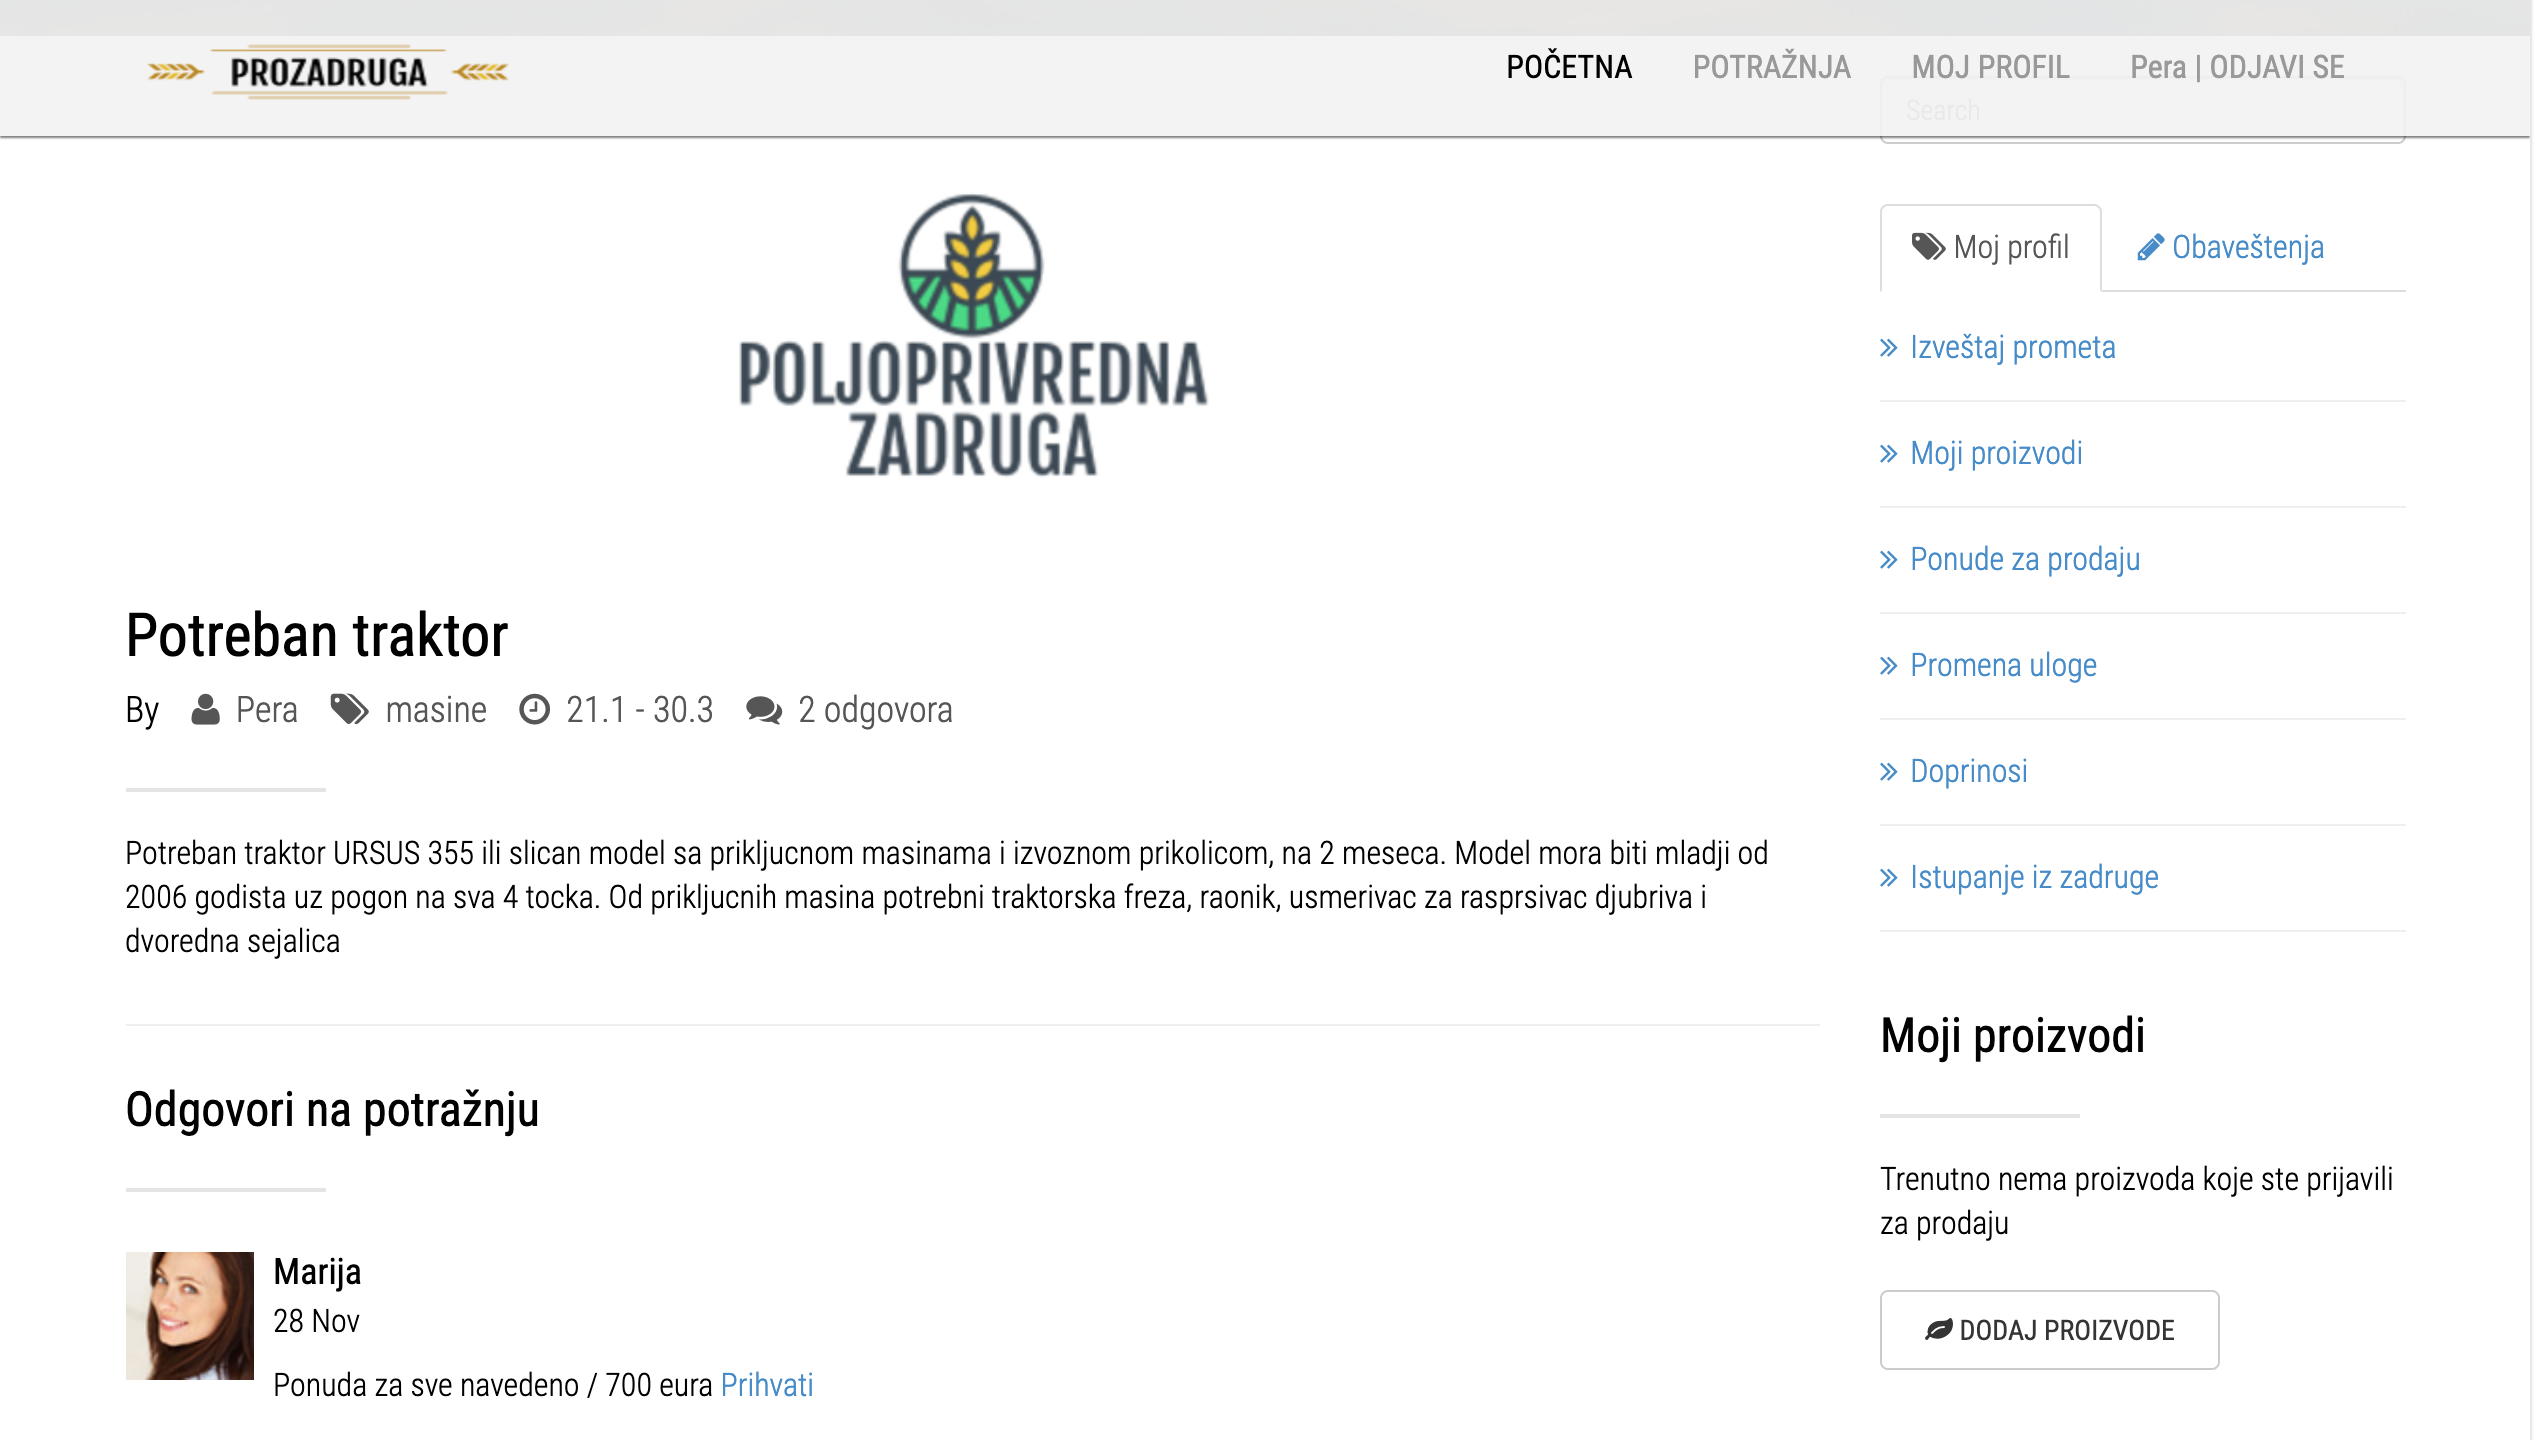
\includegraphics[scale=0.3]{images/profile2.png}
    \caption{Moj profil - opcije}
    \label{profile2}
\end{figure}

\begin{figure}[h!]
    \centering
    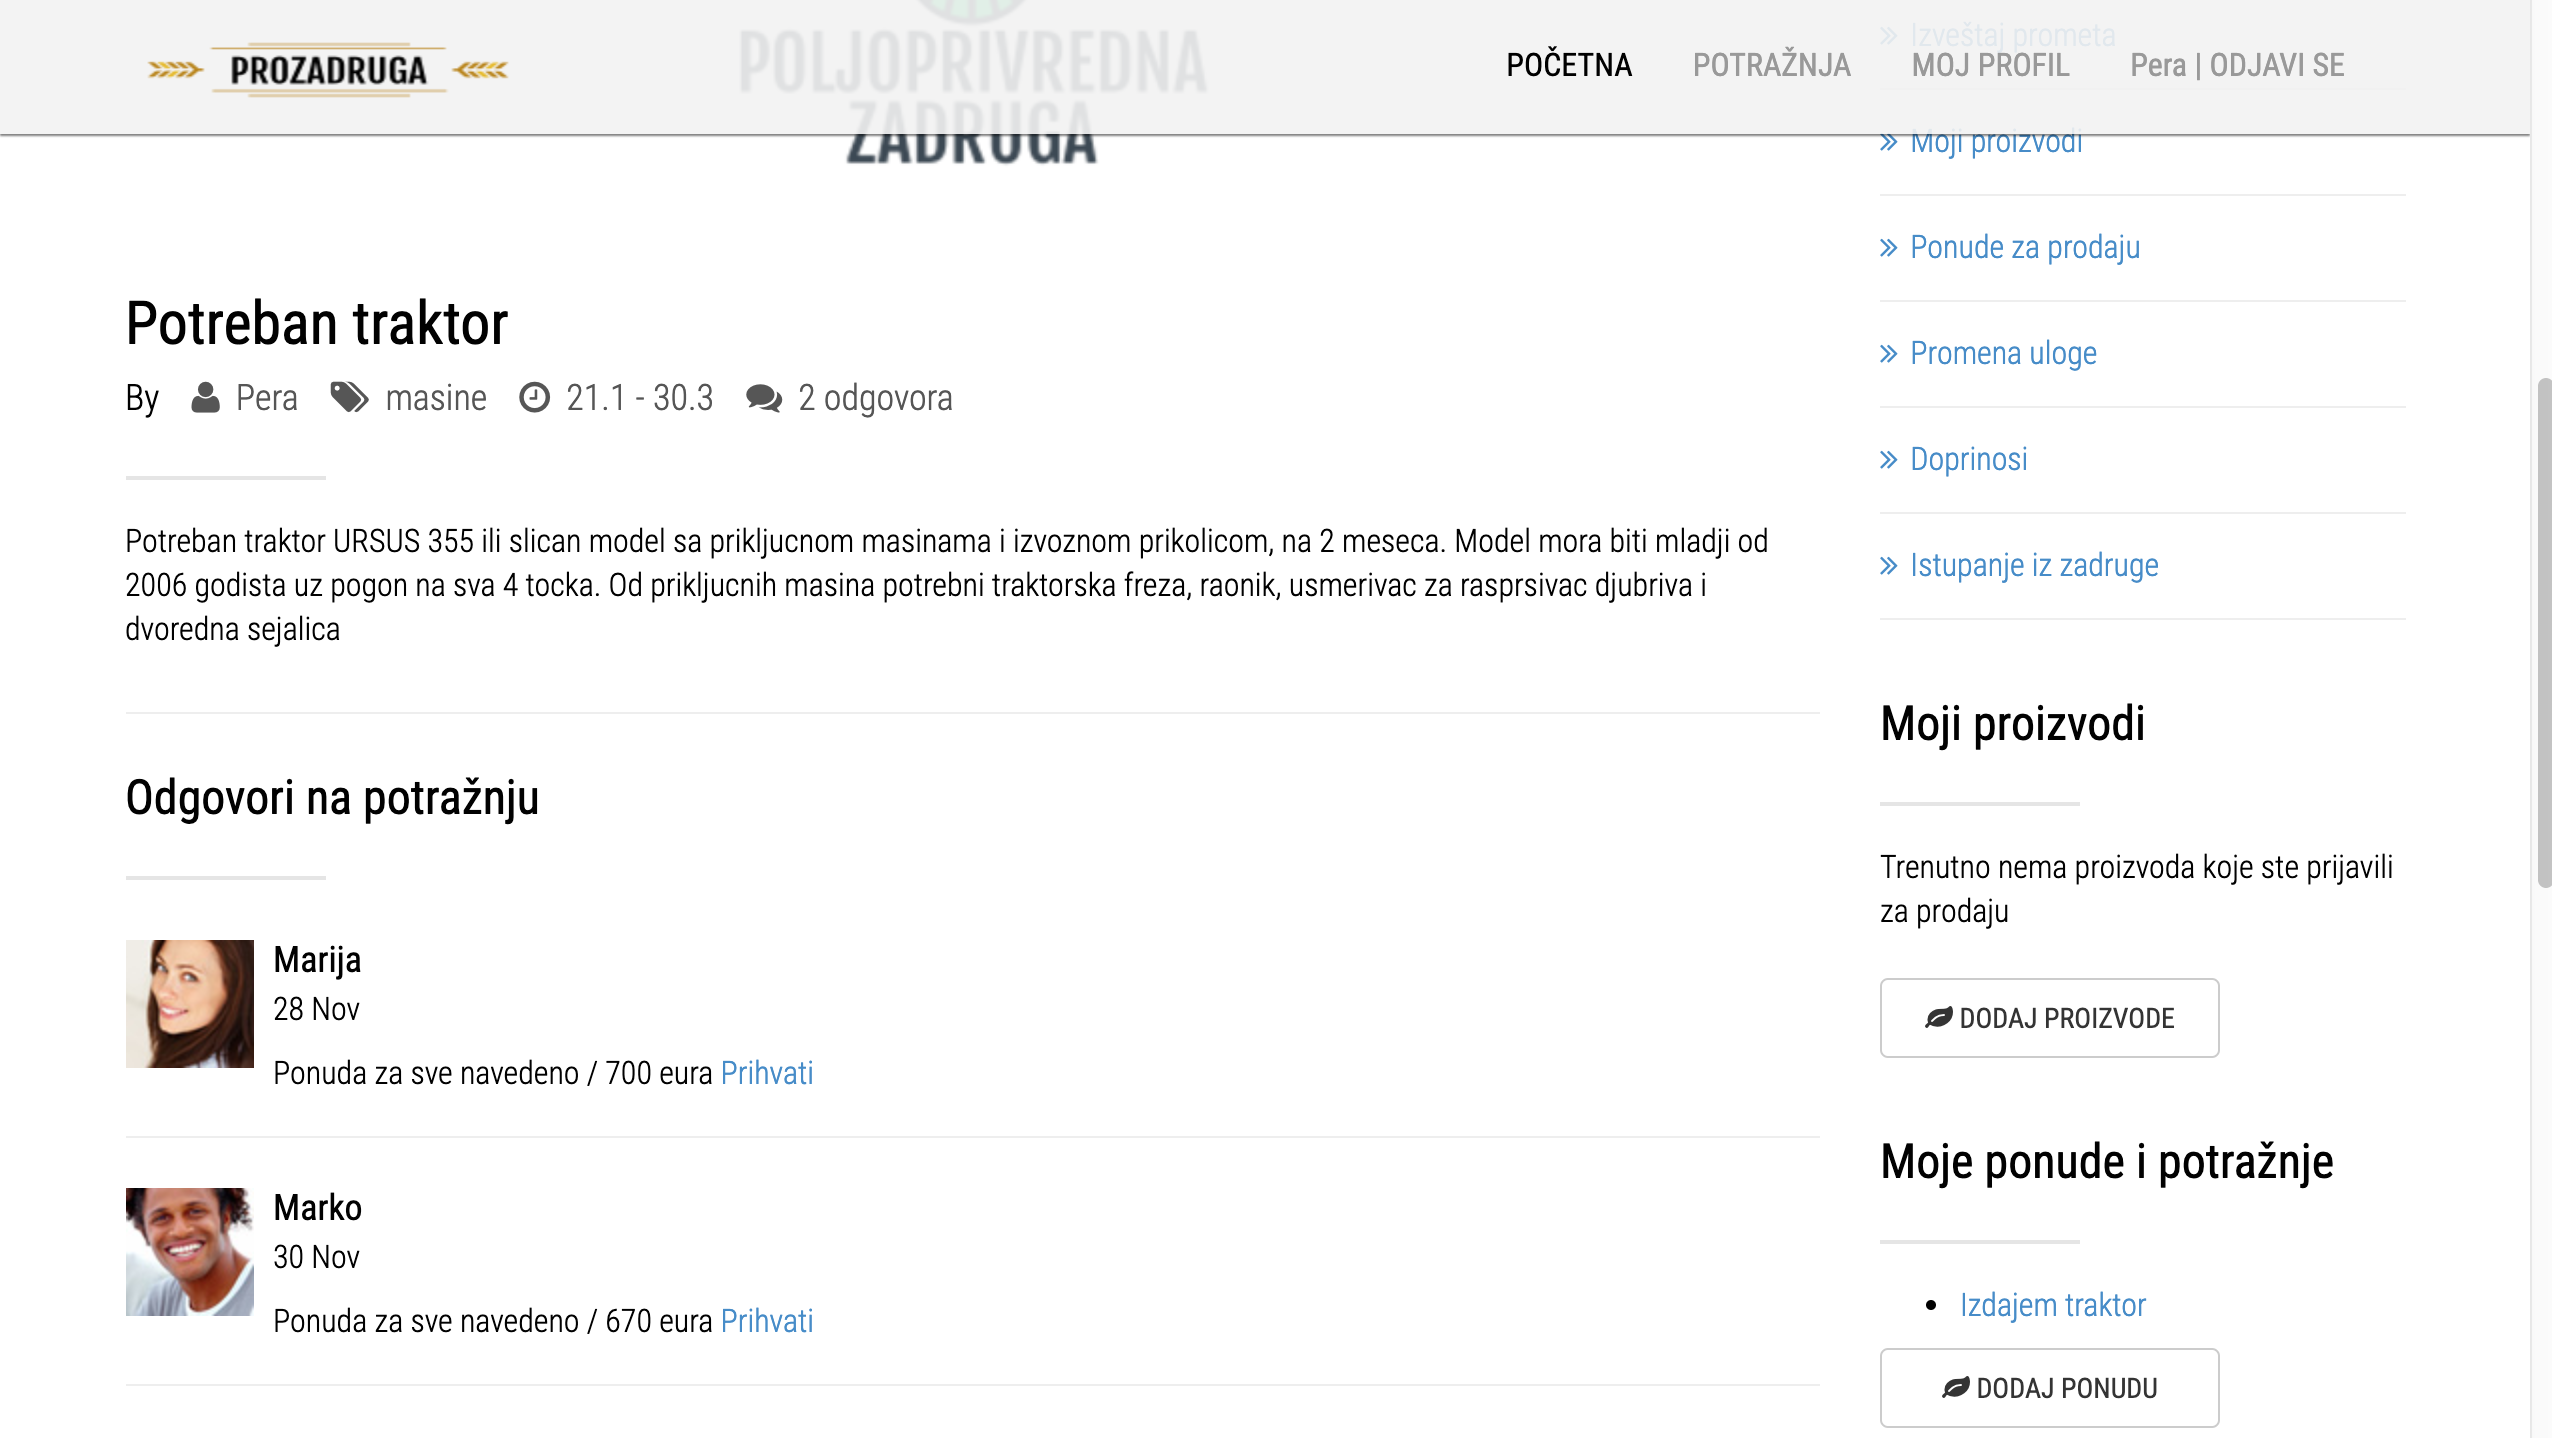
\includegraphics[scale=0.3]{images/profile3.png}
    \caption{Moj profil - potražnja}
    \label{profile3}
\end{figure}
    
\end{document}
